% Some LaTeX commands I define for my own nomenclature.
% If you have to, it's better to change nomenclature once here than in a 
% million places throughout your thesis!
%======================================================================
\chapter{Results and Discussion}
\label{c5}
%======================================================================

\section{Results for Objective 1 }
\subsection{First Task}
For Q15, do the respondents know about SafetyTips before, the result is shown in Figure~\ref{fig13}. we can find that around 50\% of the respondents from the UK and Korea do not know Safety Tips before, around 80\% of the respondents from China and Thailand know or at least heard Safety Tips before, while around 90\% of the respondents from Indonesia know or at least heard Safety Tips before. 

\begin{figure*}[h]
  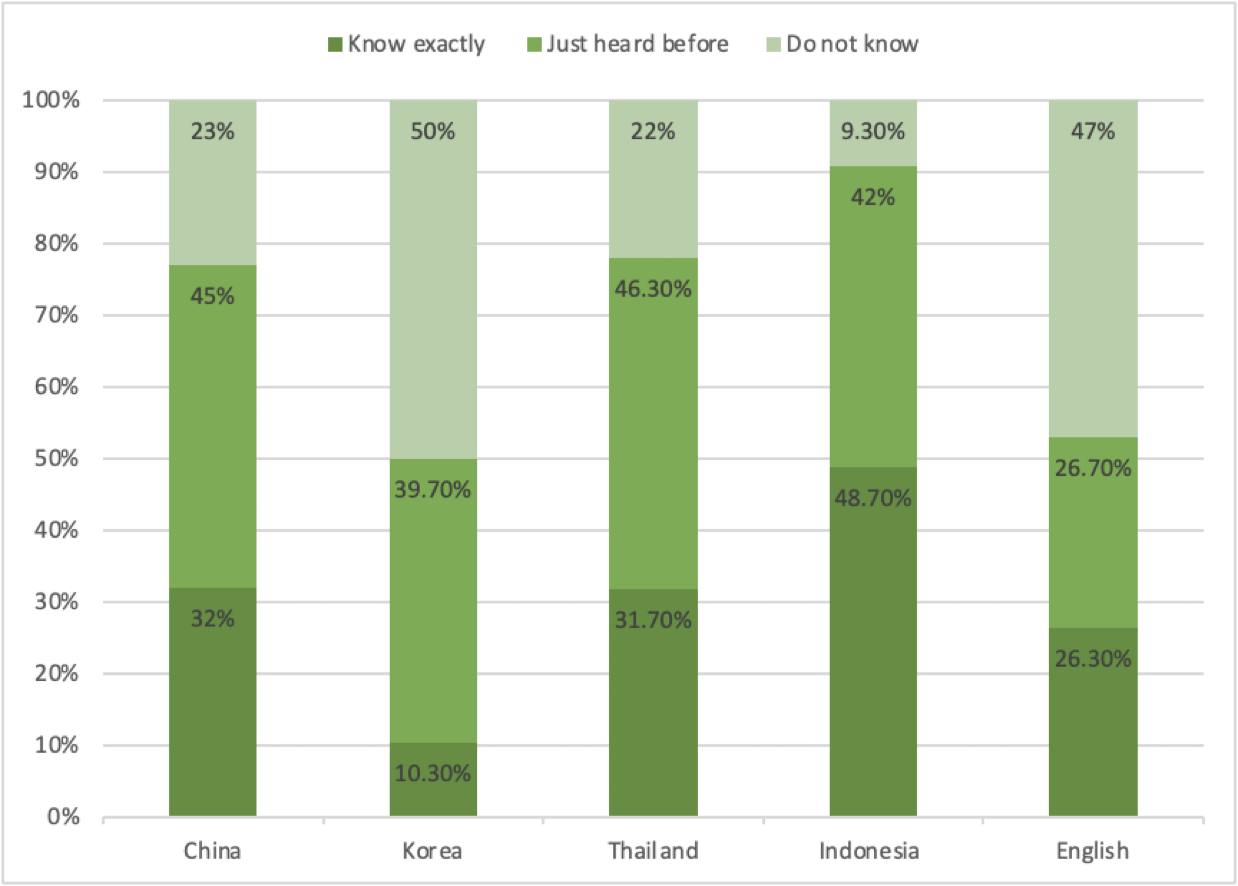
\includegraphics[width=0.8\linewidth]{Figure/Figure13.jpg}
  \centering
  \caption[Survey result of Q15]{Survey result of Q15(Do you know Safety Tips or not ?)}
  \label{fig13}
\end{figure*}

For Q16, did the respondents use SafetyTips before, the result shows in Figure~\ref{fig14}. we can find that more than 50\% of the respondents from China(66.2\%), Korea(72\%), and Thailand(55.1\%) did not use Safety Tips before, while more than 50\% of respondents from Indonesia(65.8\%) and the UK(54.7\%) have used Safety Tips before. Among all countries, respondents from Indonesia have the highest usage rate of Safety Tips at 65.8\%. Koreans had the lowest, at 28\%. 

\begin{figure*}[h]
  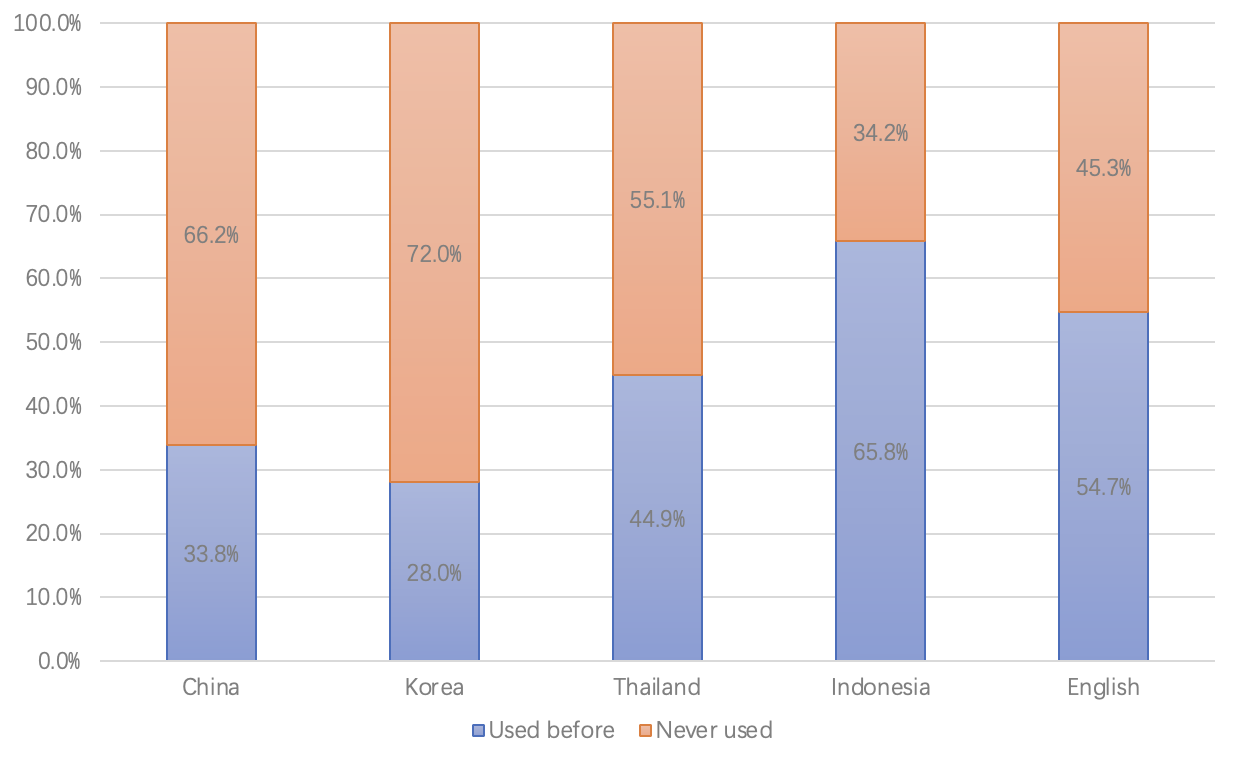
\includegraphics[width=0.8\linewidth]{Figure/Figure14.jpg}
  \centering
  \caption[Survey result of Q16]{Survey result of Q16(Do you use Safety Tips before or not ?)}
  \label{fig14}
\end{figure*}

For Q17\_1, Will the respondents trust Safety Tips more than information from their country, the result shows in Figure~\ref{fig15}. we can find that over 90\% of respondents from Thailand(91.1\%) and Indonesia(91.7\%) said they trusted information from Safety Tips more than from their own countries, and more than 80\% of respondents from China(80.3\%) feel that the information on Safety Tips could be trusted more than their own countries, while respondents from the UK(78\%) and Korea(77.3\%) have a relatively low level of trust in Safety Tips compared to the other three countries, but still around 70\%. 

\begin{figure*}[h]
  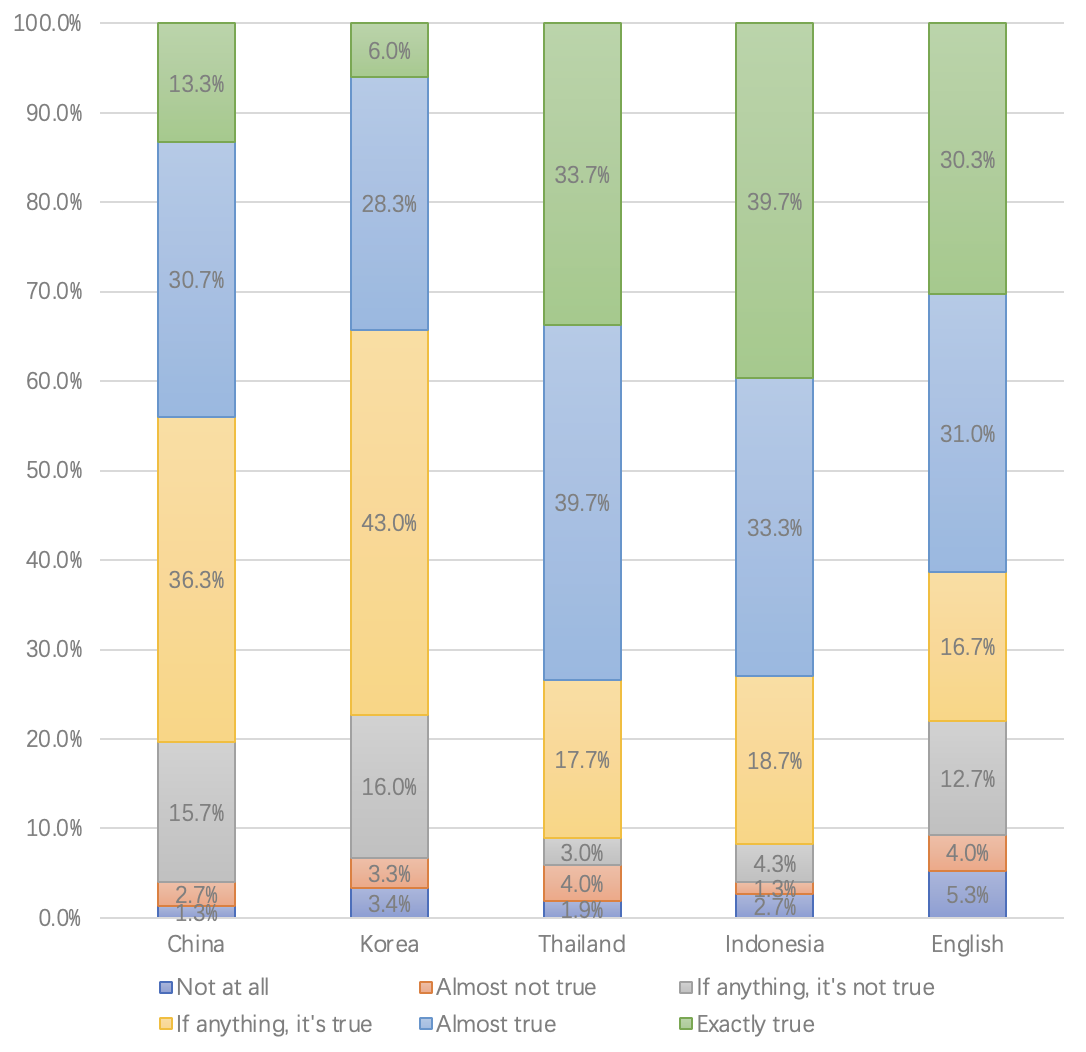
\includegraphics[width=0.8\linewidth]{Figure/Figure15.jpg}
  \centering
  \caption[Survey result of Q17\_1]{Survey result of Q17\_1(Will you trust Safety Tips more than information from your own country ?)}
  \label{fig15}
\end{figure*}

For Q17\_2, Will the respondents use Safety Tips before searching information from their country, the result shows in Figure~\ref{fig16}. we can find that over 90\% of respondents from Thailand(90.7\%) and Indonesia(94.1\%) said they use Safety Tips to search information before their own country's, and more than 80\% of respondents from China(88\%), the UK(82.3\%) and Korea(82.3\%) will use Safety Tips to find information before their own country. 

\begin{figure*}[h]
  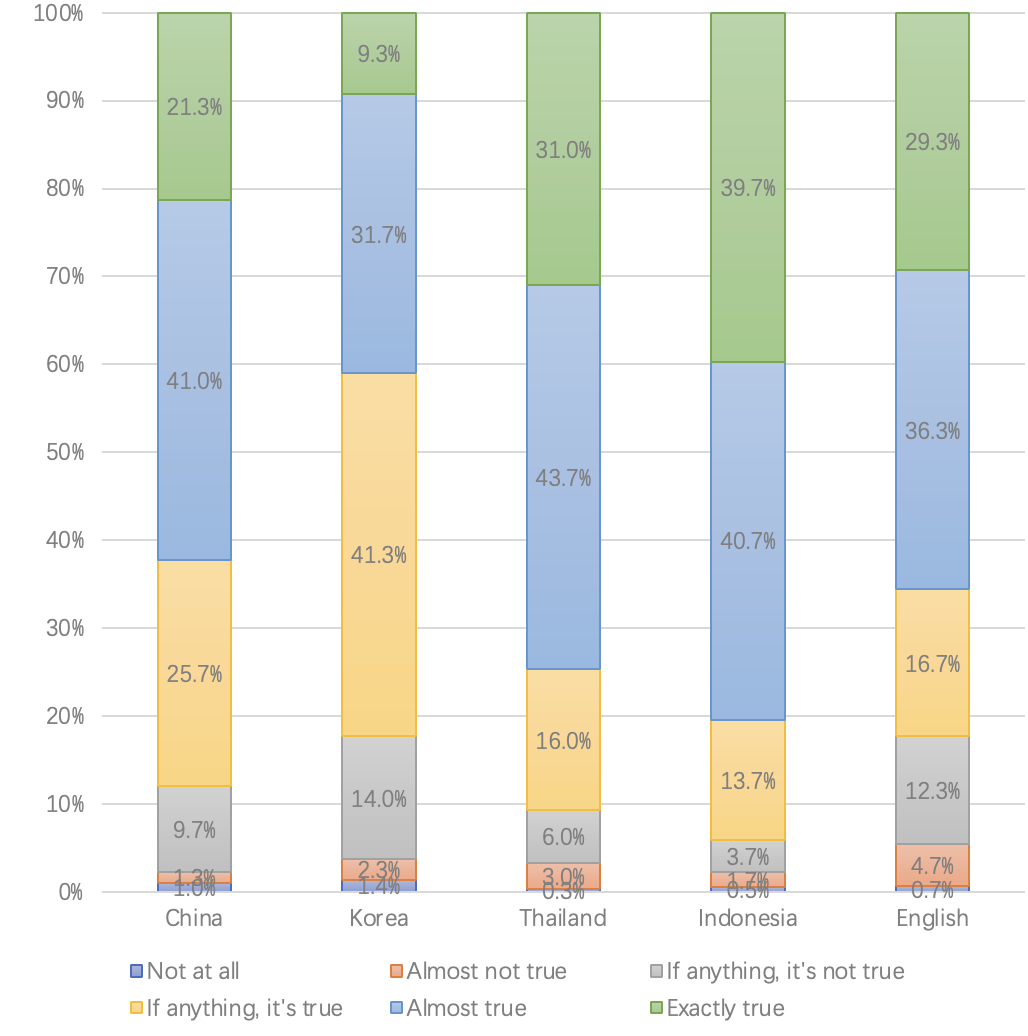
\includegraphics[width=0.8\linewidth]{Figure/Figure16.jpg}
  \centering
  \caption[Survey result of Q17\_2]{Survey result of Q17\_2(Will you use Safety Tips before searching information from your own country ?)}
  \label{fig16}
\end{figure*}

For Q17\_3, do the respondents think Safety Tips could be useful during the evacuation, the result is shown in Figure~\ref{fig17}. we can find that over 90\% of respondents from Thailand(95.4\%), China(95.7\%), and Indonesia(96.6\%) think Safety Tips could be useful during the evacuation, and more than 80\% of respondents from the UK(87\%) and Korea(84.9\%) think Safety Tips could be useful during evacuation. 

\begin{figure*}[h]
  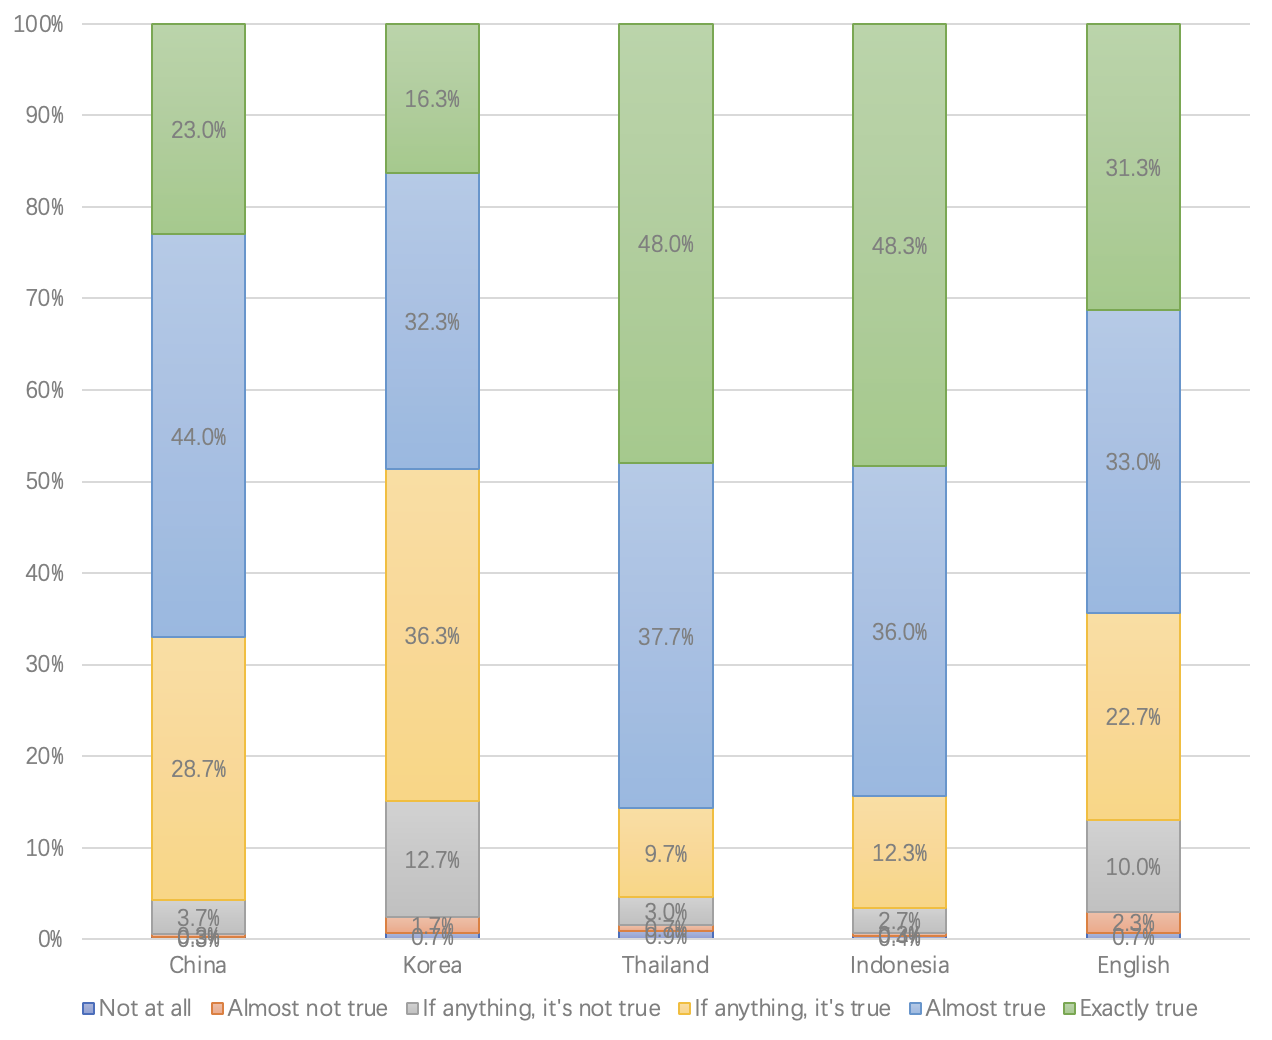
\includegraphics[width=0.8\linewidth]{Figure/Figure17.jpg}
  \centering
  \caption[Survey result of Q17\_3]{Survey result of Q17\_3(Do you think Safety Tips could be useful during evacuation ?)}
  \label{fig17}
\end{figure*}

For Q17\_4, will the respondents use Safety Tips in the future, the result shows in Figure~\ref{fig18}. we can find that over 90\% of respondents from Thailand(93.3\%), China(95.3\%), and Indonesia(95.3\%) think they will use Safety Tips in the future, and more than 80\% of respondents from the UK(87\%) and Korea(84.9\%) think they will use Safety Tips in the future.

\begin{figure*}[h]
  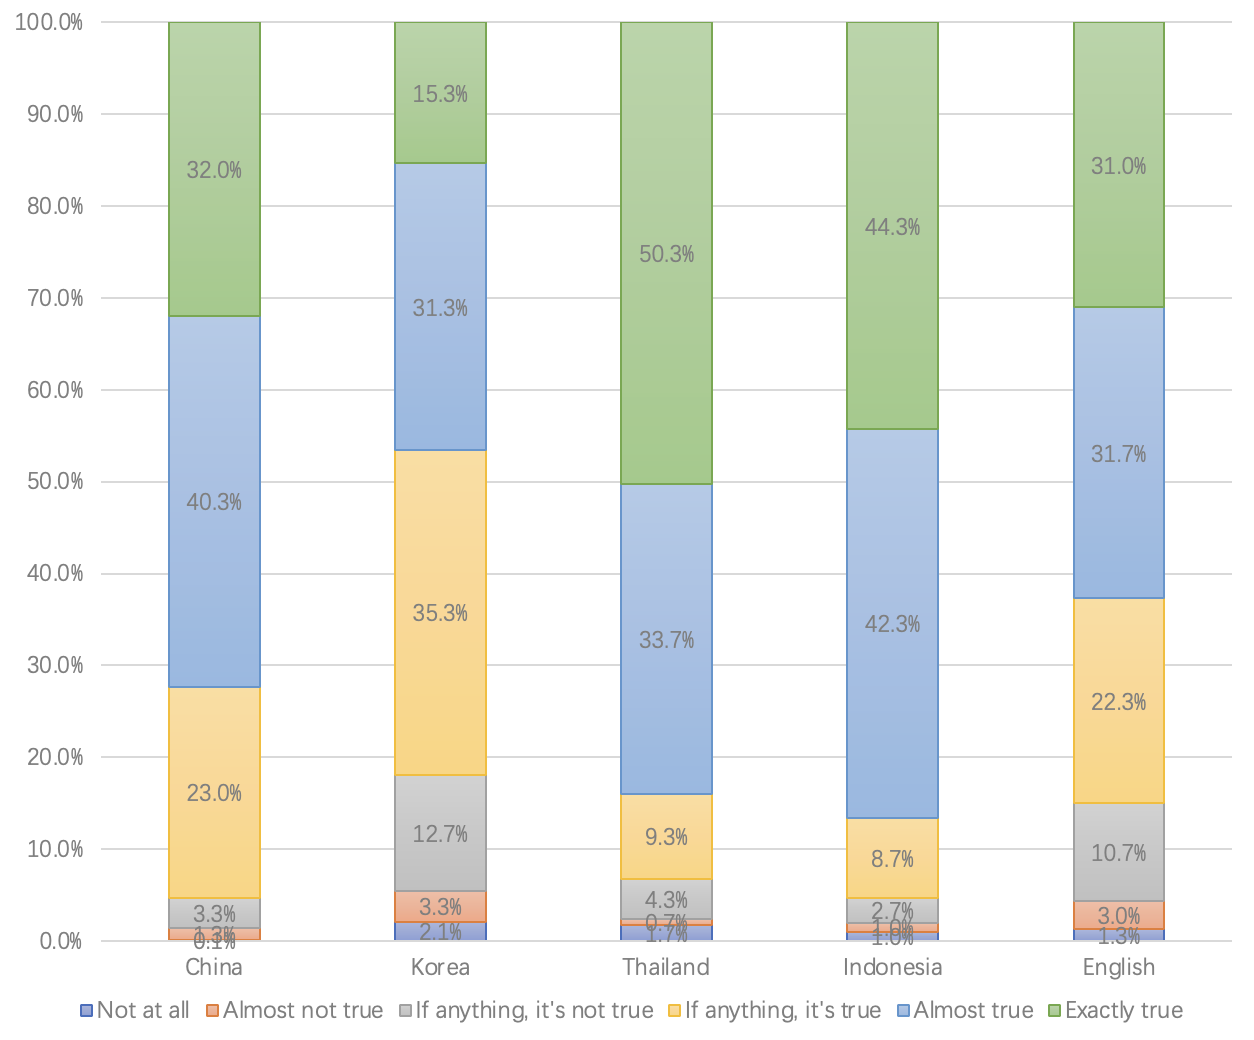
\includegraphics[width=0.8\linewidth]{Figure/Figure18.jpg}
  \centering
  \caption[Survey result of Q17\_4]{Survey result of Q17\_4(Will you use Safety Tips in the future ?)}
  \label{fig18}
\end{figure*}

From the above results, we can conclude that from the usage experience, Safety Tips could be more popular and well-known in Indonesia(90\%), China(77\%), and Thailand(79\%) rather than in the UK(53\%) and Korea(50\%). Also, among those respondents that know Safety Tips or heard them before, their usage rate is lower than 70\%. China(33.8\%), Korea(28\%), Thailand(44.9\%), Indonesia(65.8\%) and the UK(54.7\%). Then from the attitude toward Safety Tips, we can conclude that over 77\% of the respondents say that they trust Safety Tips more than information from their own countries, over 82\% of the respondents say that they will use Safety Tips to search information before from their own countries, and over 84\% of the respondents say that they believe Safety Tips could be useful during evacuation and will use Safety Tips in the future.

\subsection{Second Task}
In the second task, we aim to find whether the two factors of respondents' past awareness and whether they used it before had an impact on their attitudes toward Safety Tips. After dividing all respondents into 5 groups, we can find the differences between groups. 

First, from the results of the grouping, we can see that 80\% of those who know Safety Tips have used Safety Tips before. For those who had only heard of Safety Tips, only 22\% of the respondents had used Safety Tips before. Comparing the two sets of data, it is clear that the usage rate has decreased significantly.

For Q17\_1, Will the respondents trust Safety Tips more than information from their country, the result shows in Figure~\ref{fig19}. we can find that respondents who know exactly and used Safety Tips before have shown the highest trust toward Safety Tips, as more than 75\% of the respondents said they trust the information on Safety Tips rather than from their own countries. Respondents who know exactly but never used Safety Tips before and respondents who heard Safety Tips before but never used Safety Tips before are more likely to trust the information on Safety Tips. Respondents who heard and used Safety Tips before and respondents who do not know and never used this application before have shown a relatively negative attitude toward Safety Tips. 

\begin{figure*}[h]
  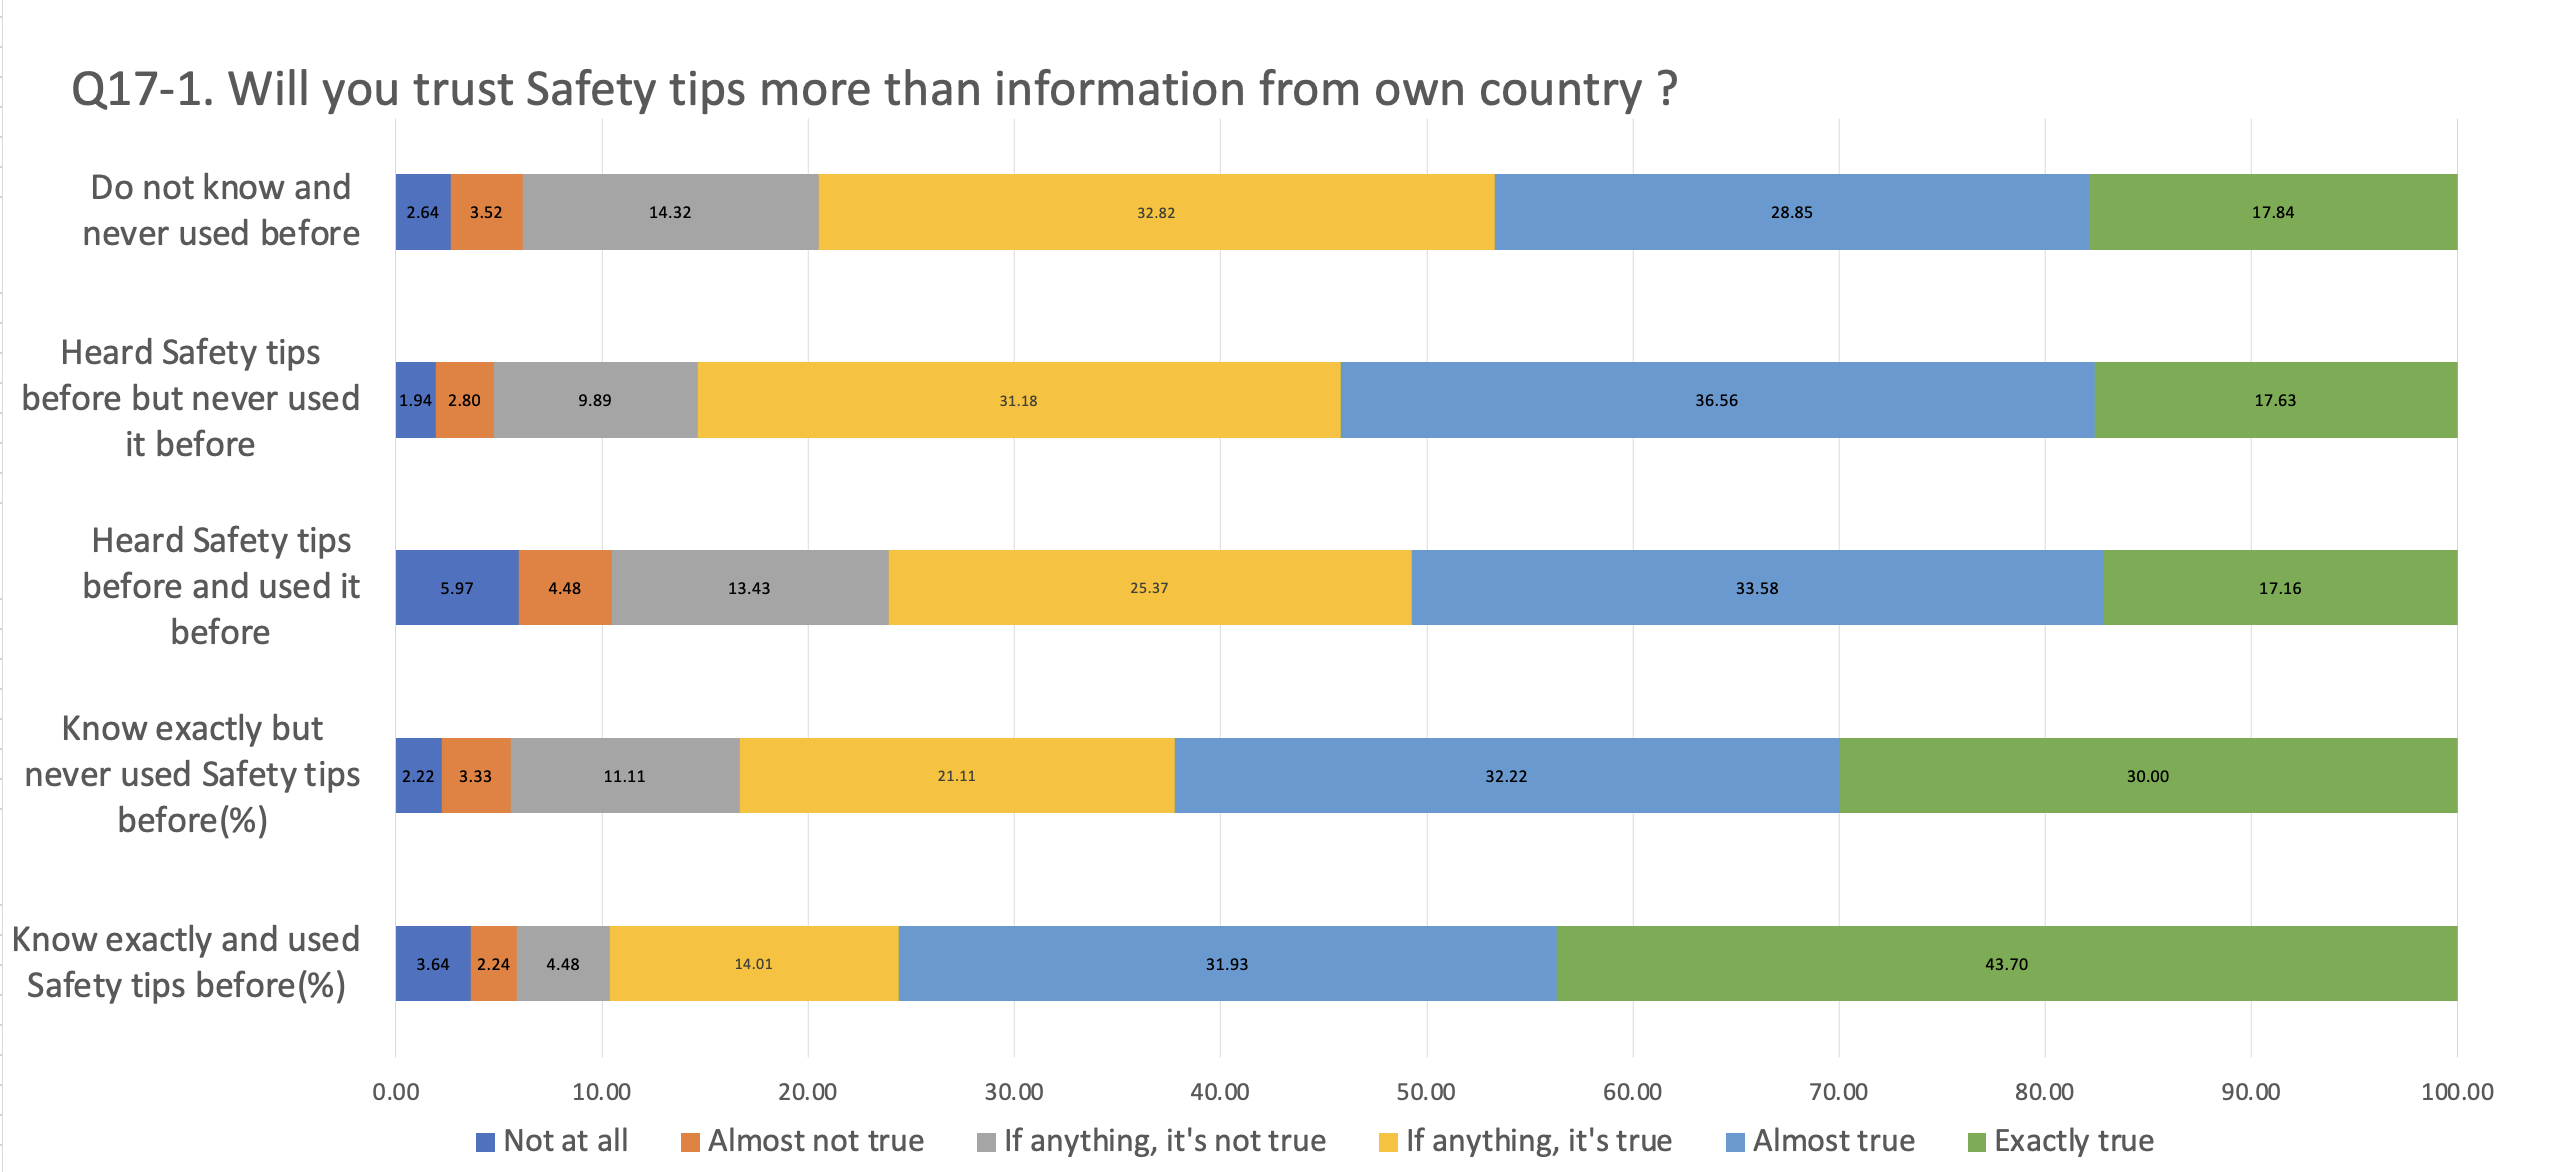
\includegraphics[width=0.8\linewidth]{Figure/Figure19.jpg}
  \centering
  \caption[5 groups of respondents' survey result of Q17\_1]{5 groups of respondents' survey result of Q17\_1(Will you trust Safety Tips more than information from your own country ?)}
  \label{fig19}
\end{figure*}

For Q17\_2, Will the respondents use Safety Tips before searching information from their country, the result shows in Figure~\ref{fig20}. we can find that the respondents who know exactly and used Safety Tips before have shown the highest usage possibility on Safety Tips, as more than 80\% of the respondents said Safety Tips have a higher priority of usage rather than from their own countries. Respondents that know exactly but never used Safety Tips before and respondents who heard Safety Tips before but never used Safety Tips before have shown similar attitudes on the priority of using Safety Tips. Respondents who do not know and never used before and respondents who heard Safety Tips before and used Safety Tips before have shown a little bit lower usage priority. 

\begin{figure*}[h]
  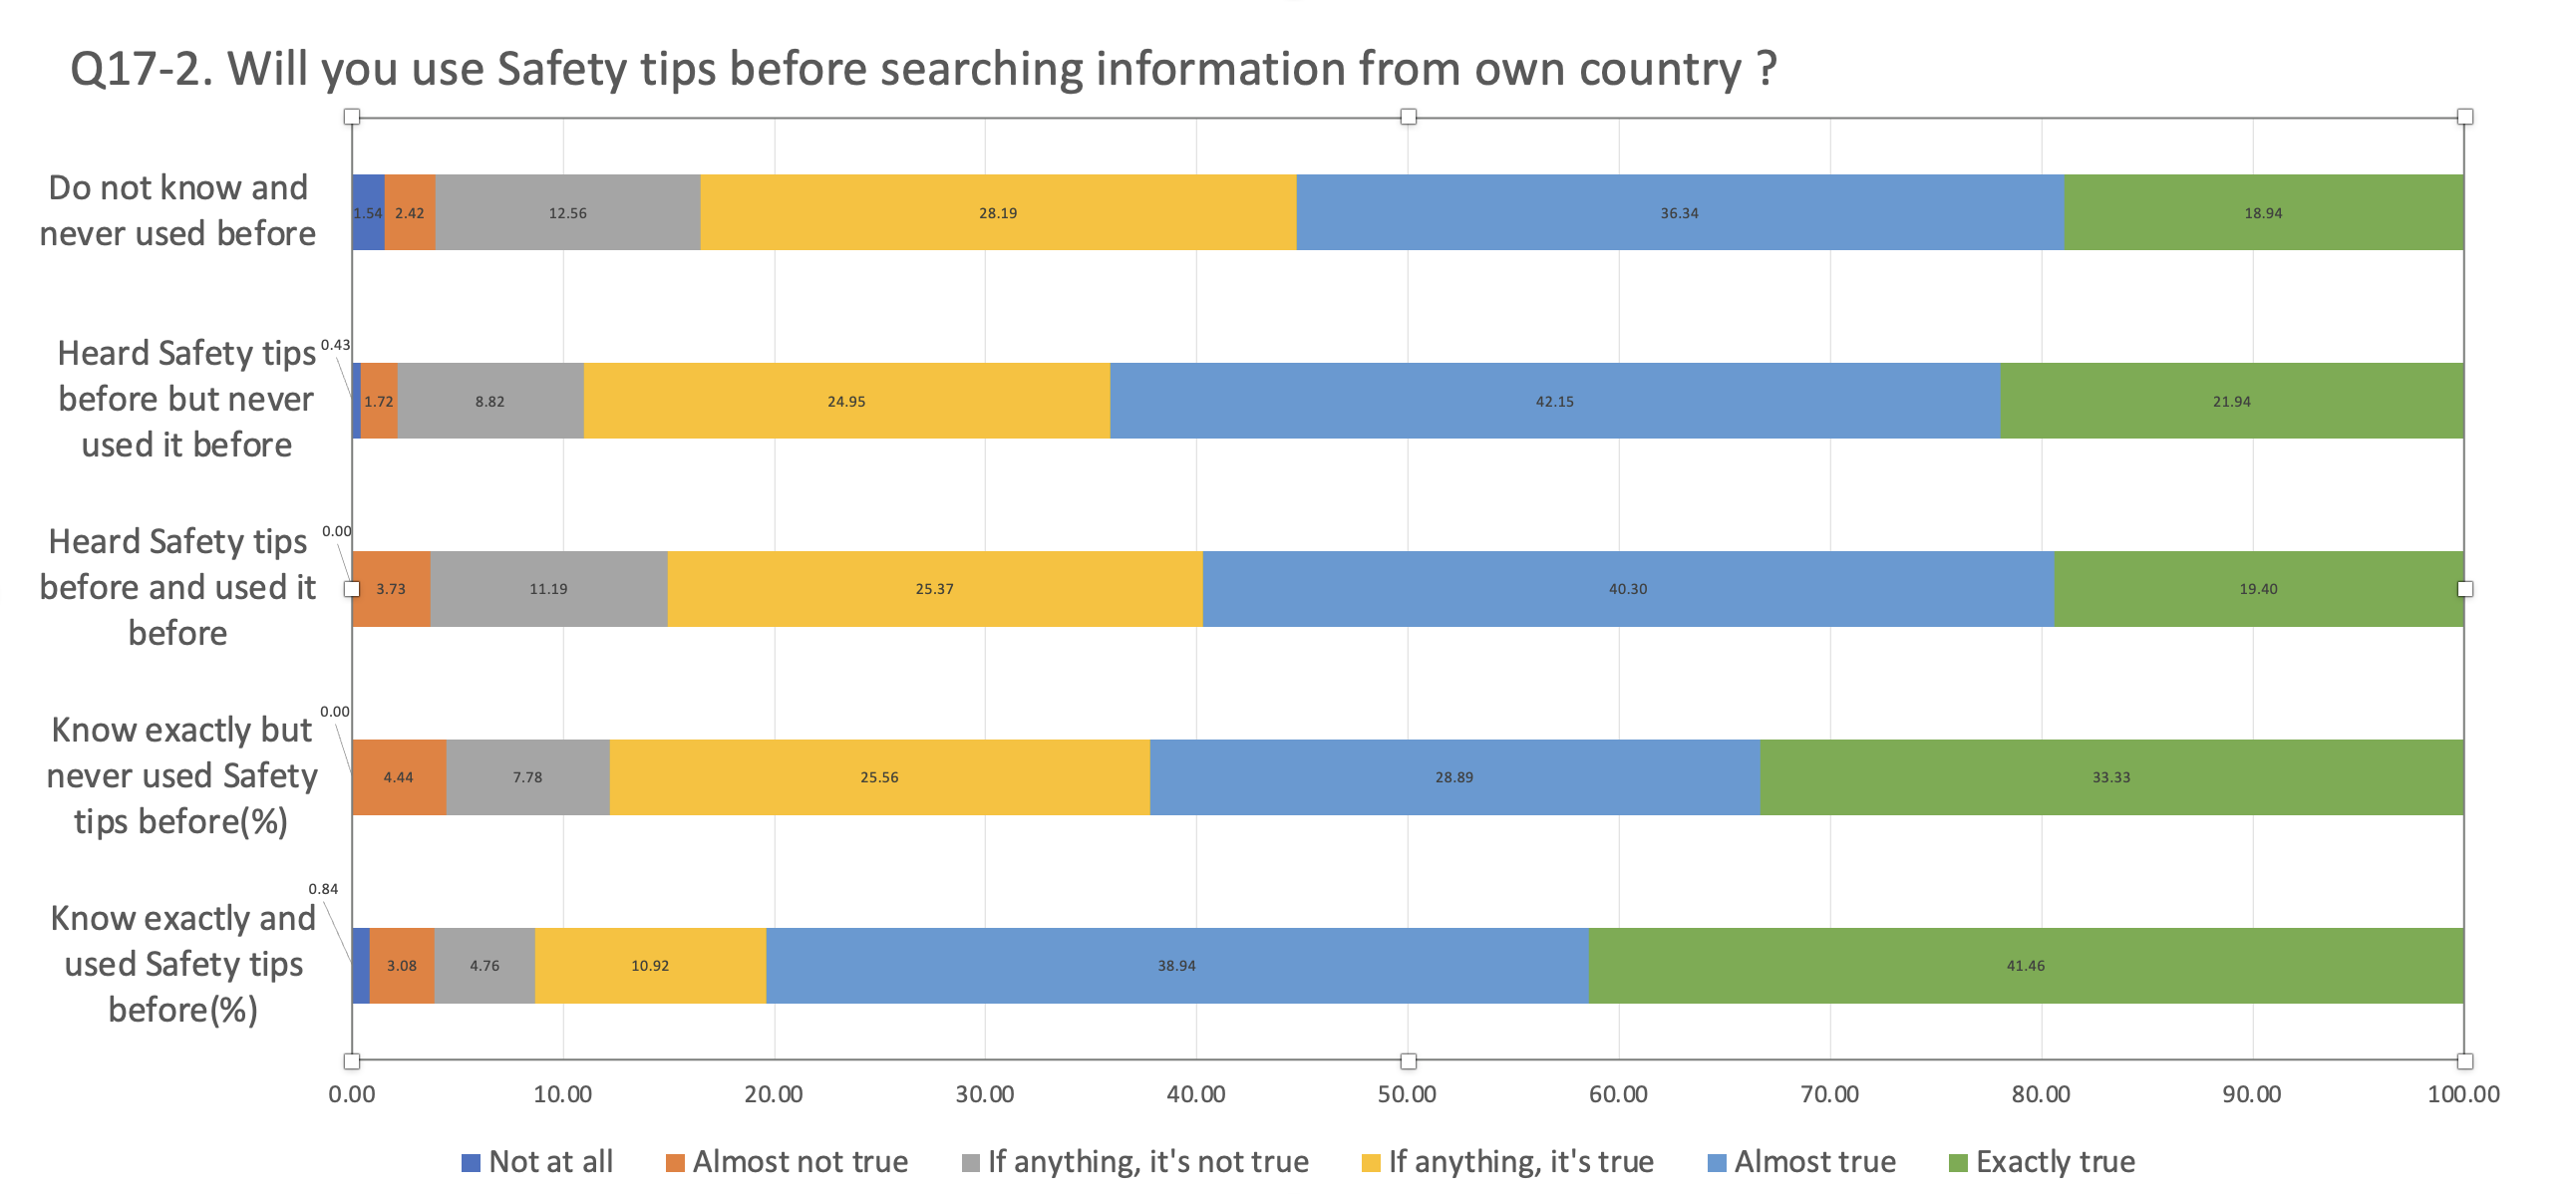
\includegraphics[width=0.8\linewidth]{Figure/Figure20.jpg}
  \centering
  \caption[5 groups of respondents' survey result of Q17\_2]{5 groups of respondents' survey result of Q17\_2(Will you use Safety Tips before searching information from your own country ?)}
  \label{fig20}
\end{figure*}

For Q17\_3, do the respondents think Safety Tips could be useful during the evacuation, the result is shown in Figure~\ref{fig21}. we can find that respondents that know exactly and used Safety Tips before and respondents who heard Safety Tips before but never used Safety Tips before could be more likely to believe Safety Tips could be useful during evacuation. Respondents that do not know and never used before, respondents who heard and used Safety Tips before, respondents who know exactly but never used Safety Tips before could be more likely to show lower usefulness of Safety Tips. 

\begin{figure*}[h]
  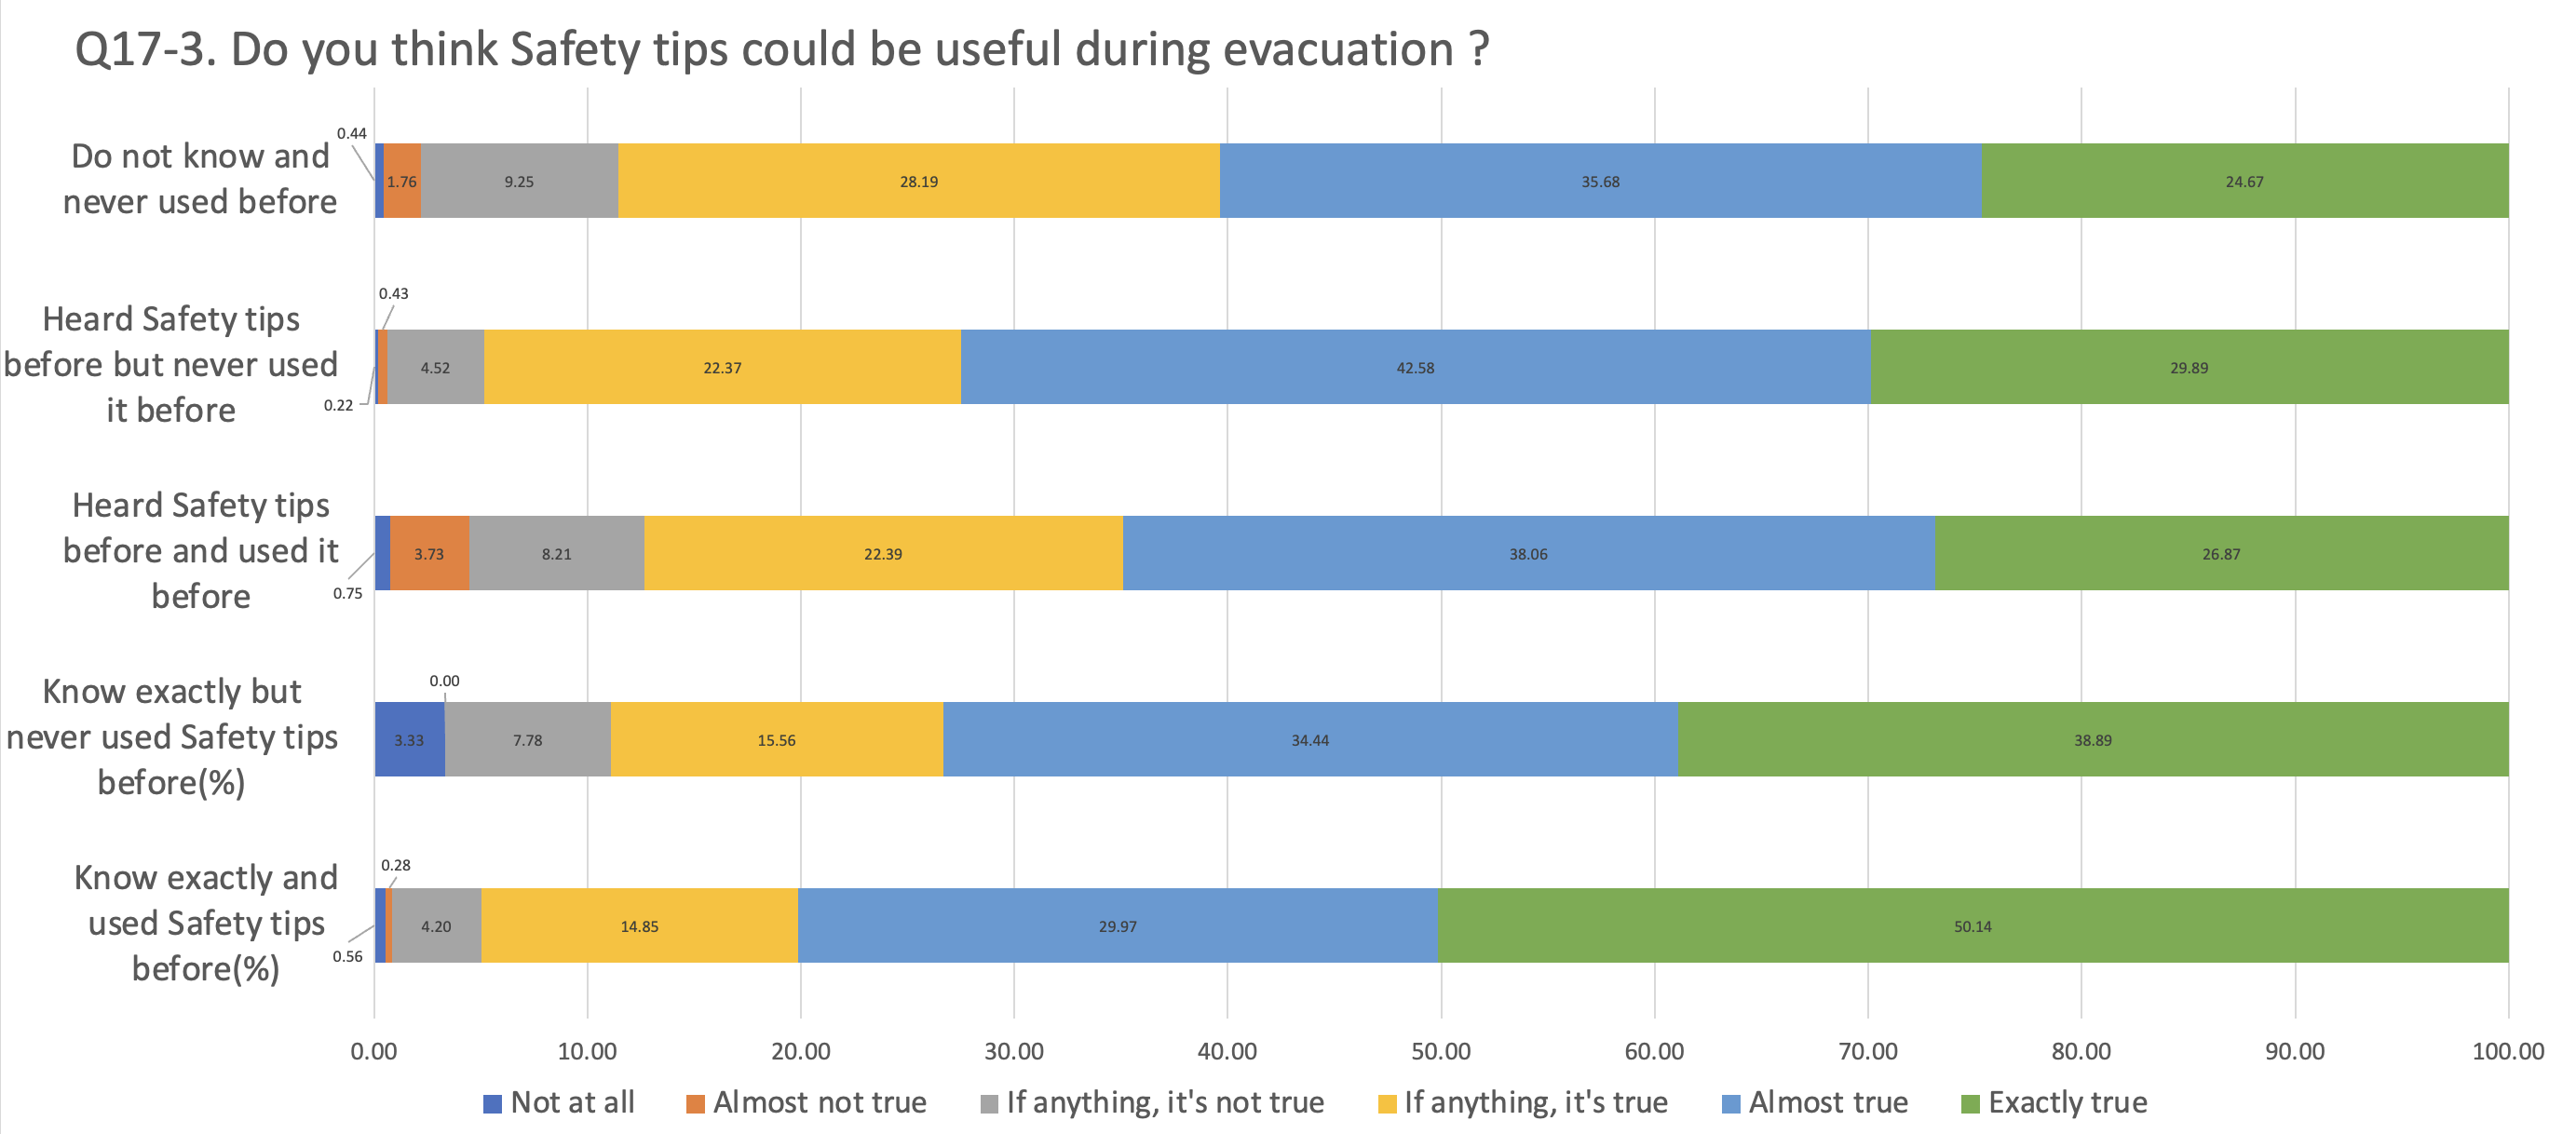
\includegraphics[width=0.8\linewidth]{Figure/Figure21.jpg}
  \centering
  \caption[5 groups of respondents' survey result of Q17\_3]{5 groups of respondents' survey result of Q17\_3(Do you think Safety Tips could be useful during evacuation ?)}
  \label{fig21}
\end{figure*}

For Q17\_4, will the respondents use Safety Tips in the future, the result shows in Figure~\ref{fig22}. we can find that respondents that know exactly and used Safety Tips before and respondents who heard but never used Safety Tips before have shown higher usage possibly Safety Tips in the future. Respondents that do not know and never used before, respondents who heard and used Safety Tips before, respondents who know exactly but never used Safety Tips before have shown relatively lower usage possibility.

\begin{figure*}[h]
  \includegraphics[width=0.8\linewidth]{Figure/Figure22.jpg}
  \centering
  \caption[5 groups of respondents' survey result of Q17\_4]{5 groups of respondents' survey result of Q17\_4(Will you use Safety Tips in the future ?)}
  \label{fig22}
\end{figure*}

From the above results, we can conclude that respondents that know exactly and used Safety Tips before could show higher trust and higher priority of use on Safety Tips, also they are more likely to believe Safety Tips can be useful during the evacuation, and they will use it in the future. And, respondents that heard but never used  Safety Tips before have shown better attitudes on Safety Tips rather than respondents who do not know and never used  Safety Tips before, respondents who heard and used Safety Tips before, respondents who know exactly but never used it Safety Tips before.

The results of the grouping indicate that 80\% of those who clearly know Safety Tips have actually used Safety Tips before. For those who had only heard of Safety Tips, only 22\% of the respondents had used Safety Tips before. Comparing the two sets of data, it is clear that the usage rate has decreased significantly. This shows that people who have a more detailed awareness of Safety Tips are more likely to use this application, so if we want to increase the usage of Safety Tips, it would be helpful to increase foreign visitors' awareness of this application.
\cleardoublepage
%%%%%%%%%%%%%%%%%%%
\section{Results for Objective 2 }
\subsection{Test for manifest variables }
Table~\ref{table27} shows the results of the statistical description with the maximum value, minimum value, mean, and standard deviation for each variable.

\begin{table}[h]
  \caption[Statistical Description]{Statistical Description (N=491)}
  \label{table27}
  \centering
  \begin{tabular}{l|cccc}
 \hline
\multicolumn{1}{c|}{Variable} & Min value  & Max value & Mean & Standard Deviation \\
 \hline
Country	& 2&6&4.32&1.30\\
gender&1&2&1.48&0.50\\
age&2&7&4.37&1.26\\
Visit\_country&1&10&4.39&2.61\\
Visit\_Japan&1&11&4.99&2.92\\
Japanese\_Level&1&4&2.59&0.77\\
Q1&1&6&4.94&1.02\\
Q2&1&6&4.95&1.01\\
Q3&1&6&5.08&0.99\\
Q4&1&6&4.55&1.03\\
Q5&1&6&3.83&1.41\\
Q6\_1\_earthquake&0&12&4.95&3.74\\
Q6\_2\_tsunami&0&12&4.53&3.33\\
Q6\_3\_typhoon&0&12&4.6&3.43\\
Q6\_4\_fire&0&12&5.01&4.06\\
Q7\_1\_earthquake&0&4&1.66&1.60\\
Q7\_2\_tsunami&0&4&0.80&1.27\\
Q7\_3\_typhoon&0&4&0.72&1.29\\
Q7\_4\_fire&0&4&1.48&1.61\\
Q8\_experience\_earthquake&1&8&3.15& 1.87\\
Q9&1&6&4.88&0.97\\
Q10	&1&6&5.01&0.95\\
Q15 Safetytips&2&3&2.73&0.45\\
Q16 Safetytips\_use&1&1&1&0\\
Q17 Safetytips\_trust\_1&1&6&4.8&1.31\\
Q17 Safetytips\_trust\_2&1&6&4.95&1.08\\
Q17 Safetytips\_trust\_3&1&6&5.10&1.01\\
Q17 Safetytips\_trust\_4&1&6&5.11&1.02\\
 \hline
  \end{tabular}
\end{table}

For some group-based data, the frequency descriptions of these variables are shown in the following. \crefrange{table28a}{table28f} is the frequency description of Item 1, including Country, Gender, Age, number of visited countries, number of visited Japan, Japanese Level. Table~\ref{table28g} is the frequency description of Item 3, that is the severity of the earthquake experience.

\begin{table}[h]
  \caption[Frequency Description of Country]{Frequency Description of Country (N=491)}
  \label{table28a}
  \centering
  \begin{tabular}{l|cc}
 \hline
\multicolumn{1}{c|}{Category}&Number&Rate\\
 \hline
China&78&15.90\%\\
South Korea&42&8.60\%\\
Thailand&105&21.40\%\\
Indonesia&179&36.50\%\\
the UK&87&17.70\%\\
 \hline
  \end{tabular}
\end{table}

\begin{table}[h]
  \caption[Frequency Description of Gender]{Frequency Description of Gender (N=491)}
  \label{table28b}
  \centering
  \begin{tabular}{l|cc}
 \hline
\multicolumn{1}{c|}{Category}&Number&Rate\\
 \hline
Male   & 253 & 51.50\% \\
Female & 238 & 48.50\% \\
 \hline
  \end{tabular}
\end{table}

\begin{table}[h]
  \caption[Frequency Description of Age]{Frequency Description of Age (N=491)}
  \label{table28c}
  \centering
  \begin{tabular}{l|cc}
 \hline
\multicolumn{1}{c|}{Category}&Number&Rate\\
 \hline
Age 16-19   & 13  & 2.60\%  \\
Age 20-29   & 136 & 27.70\% \\
Age 30-39   & 126 & 25.70\% \\
Age 40-49   & 113 & 23\%    \\
Age 50-59   & 77  & 15.70\% \\
Age 60-69   & 26  & 5.30\%  \\
Age over 70 & 0   & 0\% \\
 \hline
  \end{tabular}
\end{table}

\begin{table}[h]
  \caption[Frequency Description of number of visited country ]{Frequency Description of number of visited country (N=491)}
  \label{table28d}
  \centering
  \begin{tabular}{l|cc}
 \hline
\multicolumn{1}{c|}{Category}&Number&Rate\\
 \hline
0 time        & 0                    & 0\%                  \\
1 time        & 73                   & 14.90\%              \\
2 times       & 63                   & 12.80\%              \\
3 to 4 times  & 152                  & 31\%                 \\
5 to 6 times  & 95                   & 19.30\%              \\
7 to 9 times  & 99                   & 20.20\%              \\
Over 10 times & 9                    & 1.80\%               \\
 \hline
  \end{tabular}
\end{table}

\begin{table}[h]
  \caption[Frequency Description of number of visited Japan]{Frequency Description of number of visited Japan (N=491)}
  \label{table28e}
  \centering
  \begin{tabular}{l|cc}
 \hline
\multicolumn{1}{c|}{Category}&Number&Rate\\
 \hline
0 time        & 0   & 0\%     \\
1 time        & 47  & 9.60\%  \\
2 times       & 65  & 13.20\% \\
3 to 4 times  & 147 & 29.90\% \\
5 to 6 times  & 85  & 17.30\% \\
7 to 9 times  & 81  & 16.50\% \\
Over 10 times & 66  & 13.40\% \\
 \hline
  \end{tabular}
\end{table}

\begin{table}[h]
  \caption[Frequency Description of Japanese Level]{Frequency Description of Japanese Level (N=491)}
  \label{table28f}
  \centering
  \begin{tabular}{l|cc}
 \hline
\multicolumn{1}{c|}{Category}&Number&Rate\\
 \hline
Cannot understand                    & 25  & 5.10\%  \\
Basic        & 214 & 43.60\% \\
Intermediate & 190 & 38.70\% \\
Up level     & 62  & 12.60\% \\
 \hline
  \end{tabular}
\end{table}

\begin{table}[h]
  \caption[Frequency Description of severity of the earthquake experienced]{Frequency Description of severity of the earthquake experienced (N=491)}
  \label{table28g}
  \centering
  \begin{tabular}{l|cc}
 \hline
\multicolumn{1}{c|}{Category}&Number&Rate\\
 \hline
MMI intensity 5 or less / intensity 3 or less & 110 & 22.40\% \\
MMI intensity 6 / intensity 4                 & 90  & 18.30\% \\
MMI intensity 7 / intensity 5 weak            & 119 & 24.20\% \\
MMI intensity 8 / intensity 5 strong          & 80  & 16.30\% \\
MMI intensity 9 / intensity 6 weak            & 30  & 6.10\%  \\
MMI intensity 10 / intensity 6 strong                                 & 18  & 3.70\%  \\
MMI intensity 11 to 12 / intensity 7                                  & 30  & 6.10\%  \\
no earthquake experience                                              & 14  & 2.90\%  \\
 \hline
  \end{tabular}
\end{table}

For the scale questions in the questionnaire, we conducted a one-sample t-test, and the results of the study can indicate whether people have clear attitudes in their responses to these questions. For question Q17 about the attitude toward Safety Tips, the answers to the scale questions were divided into 6 dimensions, so we set 3.5 as the test value. Table~\ref{table29} shows the results of the one-sample t-test. For Q17\_1 to Q17\_1, the mean values of 491 respondents are 4.80$\pm$1.31; 4.95$\pm$1.08; 5.10$\pm$1.01; 5.11$\pm$1.02; All of the p values are less than 0.01, mean all are statistically significant at $p<0.001$ level. Compared to the test value of 3.5, indicating that all have significant differences in the attitude toward Safety Tips, and all mean values are higher than the test value of 3.5, implying that respondents show positive attitudes to all of the questions towards Safety Tips. 

\begin{table}[h]
  \caption[Result of one-sample t-test]{Result of one-sample t-test (N=491)}
  \label{table29}
  \centering
  \begin{tabular}{l|cccc}
 \hline
                  & Mean                 & Test Value & t                          & p                        \\
Q17Safetytips\_trust\_1 & 4.80$\pm$1.31            & 3.5                            & 29.96 & 0.00 \\
Q17Safetytips\_trust\_2 & 4.95$\pm$1.08            & 3.5                            & 29.96 & 0.00 \\
Q17Safetytips\_trust\_3 & 5.10$\pm$1.01            & 3.5                            & 35.18 & 0.00 \\
Q17Safetytips\_trust\_4 & 5.11$\pm$1.02            & 3.5                            & 34.81 & 0.00 \\
 \hline
  \end{tabular}
\end{table}

On the other hand, this study also used the Chi-squared test and ANOVA to test whether those manifest variables could show significant differences in respondents' attitudes towards Safety Tips. Table~\ref{table30} shows the statistical results of the sample data for the manifest variable Gender and the four attitude-related questions in Q17. We can see that in Q17\_2/3/4, there are less than 5 male and female respondents. Therefore, in order to observe the significant differences more clearly, here we group the Q17 answers into two categories, 1 to 3 as negative attitude and 4 to 6 as a positive attitude. \crefrange{table31a}{table31d} show the Chi-squared test results. From the results, we find that the p-values between gender and all four attitude related questions are bigger than 0.05, (gender*Q17\_1: $p=0.525>0.05$; gender*Q17\_2: $p=0.705>0.05$; gender*Q17\_3: $p=0.490>0.05$; gender*Q17\_4: $p=0.852>0.05$;)which indicates that gender differences are not significantly different in Q17's responses. 

\begin{table}[h]
  \caption{Sample data of Gender*Q17}
  \label{table30}
  \centering
\begin{tabular}{cc|ccccccc}
\hline
Question & Answer & 1  & 2  & 3  & 4  & 5   & 6   & Total \\
\hline
\multirow{3}{*}{Q17\_1}   & Female & 10 & 6  & 15 & 34 & 76  & 97  & 238                       \\
         & Male   & 11 & 8  & 19 & 50 & 83  & 82  & 253                       \\
         & Total  & 21 & 14 & 34 & 84 & 159 & 179 & 491                       \\
\hline
\multirow{3}{*}{Q17\_2}   & Female & 0  & 9  & 17 & 23 & 108 & 81  & 238                       \\
         & Male   & 3  & 7  & 15 & 50 & 85  & 93  & 253                       \\
         & Total  & 3  & 16 & 32 & 73 & 193 & 174 & 491                       \\
\hline
\multirow{3}{*}{Q17\_3}   & Female & 0  & 2  & 13 & 34 & 73  & 116 & 238                       \\
         & Male   & 3  & 4  & 13 & 49 & 85  & 99  & 253                       \\
         & Total  & 3  & 6  & 26 & 83 & 158 & 215 & 491                       \\
\hline
\multirow{3}{*}{Q17\_4}   & Female & 2  & 3  & 10 & 25 & 91  & 107 & 238                       \\
         & Male   & 4  & 5  & 8  & 46 & 89  & 101 & 253                       \\
         & Total  & 6  & 8  & 18 & 71 & 180 & 208 & 491                     \\
\hline         
\end{tabular}
\end{table}

\begin{table}[h]
  \caption{Chi-square test result of Gender*Q17\_1 }
  \label{table31a}
  \centering
\begin{tabular}{c|ccc}
\hline
Gender & negative & positive & Total \\
\hline
Female & 31                           & 207                          & 238                       \\
Male   & 38                           & 215                          & 253                       \\
Total  & 69                           & 422                          & 491                       \\
\hline
p-value      &        &      & 0.525   \\
\hline                   
\end{tabular}
\end{table}

\begin{table}[h]
  \caption{Chi-square test result of Gender*Q17\_2 }
  \label{table31b}
  \centering
\begin{tabular}{c|ccc}
\hline
Gender & negative & positive & Total \\
\hline
Female & 26                           & 212                          & 238                       \\
Male   & 25                          & 228                         & 253                       \\
Total  & 51                           & 440                          & 491                       \\
\hline
p-value      &        &      & 0.705   \\
\hline                   
\end{tabular}
\end{table}

\begin{table}[h]
  \caption{Chi-square test result of Gender*Q17\_3 }
  \label{table31c}
  \centering
\begin{tabular}{c|ccc}
\hline
Gender & negative & positive & Total \\
\hline
Female & 15                           & 223                          & 238                       \\
Male   & 20                          & 233                       & 253                       \\
Total  & 35                           & 456                          & 491                       \\
\hline
p-value     &        &      & 0.490   \\
\hline                   
\end{tabular}
\end{table}

\begin{table}[h]
  \caption{Chi-square test result of Gender*Q17\_4 }
  \label{table31d}
  \centering
\begin{tabular}{cccc}
\hline
Gender & negative & positive & Total \\
\hline
Female & 15                           & 223                          & 238                       \\
Male   & 17                         & 236                      & 253                       \\
Total  & 32                           & 459                          & 491                       \\
\hline
p-value      &        &      & 0.852   \\
\hline                   
\end{tabular}
\end{table}

\crefrange{table32a}{table32e} shows the ANOVA results of age, number of visited countries, number of visited Japan, Japanese level, the severity of the earthquake experienced. Through ANOVA, we analyzed several manifest variables for the test of differences in attitudes. The results of Table~\ref{table32a} shows that as p-value is less than 0.05 for the first three questions (age*Q17\_1: $p=0.000<0.05$; age*Q17\_2: $p=0.035<0.05$; age*Q17\_3: $p=0.000<0.05$), the age difference is significantly different on their attitudes toward Safety Tips . However, for the possibility of future use, there is no significant difference because p is bigger than 0.05 (age*Q17\_4: $p=0.076>0.05$). For these first three questions with significant differences, the mean values were able to give the following results. For trust level, the older the age, the more positive the attitude. For the priority of use, the attitudes of the respondents from Age 20 to 39 are lower than those of the other age groups, and from Age over 40, the attitudes tend to change more positively with age. For usefulness, the results do not show any tendency to change. However, Age 60 to 69 respondents gave the most positive attitudes, while Age 30 to 39 respondents had the most negative attitudes on average. The results of Table~\ref{table32b} show that the differences in the number of visited countries do not reflect significant differences in trust level and priority of use because the p-values for the first two questions are bigger than 0.05 (number of visited countries*Q17\_1: $p=0.140>0.05$; the number of visited countries*Q17\_2: $p=0.270>0.05$;). However, for usefulness and Possibility of future use, there are significant differences since the p-value is less than 0.05 (number of visited countries*Q17\_3: $p=0.009<0.05$; the number of visited countries*Q17\_4: $p=0.049<0.05$;). For these two questions with significant differences, the mean results did not show any tendency, however, the respondents with more than 5 visits could have better attitudes. The results of Table~\ref{table32c} shows that the p-value for each question is less than 0.05 (number of visited Japan*Q17\_1: $p=0.000<0.05$; the number of visited Japan*Q17\_2: $p=0.002<0.05$; the number of visited Japan*Q17\_3: $p=0.000<0.05$; the number of visited Japan*Q17\_4: $p=0.000<0.05$;), so the difference in the Number of visited Japan reflects a significant difference in the responses to attitudes toward Safety Tips. The average results show that the more the number of visits to Japan, the more positive the respondents' attitudes toward Safety Tips. The results of Table~\ref{table32d} shows that the p-value for each question is less than 0.05 (Japanese level*Q17\_1: $p=0.000<0.05$; Japanese level*Q17\_2: $p=0.032<0.05$; Japanese level*Q17\_3: $p=0.000<0.05$; Japanese level*Q17\_4: $p=0.021<0.05$;), so the difference in Japanese language proficiency is reflected in the significant difference in the attitudes toward Safety Tips responses. The results of the averages basically show that the higher the Japanese language level, the more positive the attitudes toward Safety Tips of the respondents. The results of Table~\ref{table32e} show that the p-value for each question is greater than 0.05 (severity of experienced earthquakes*Q17\_1: $p=0.548>0.05$; severity of experienced earthquakes*Q17\_2: $p=0.127>0.05$; severity of experienced earthquakes*Q17\_3: $p=0.389>0.05$; severity of experienced earthquakes*Q17\_4: $p=0.121>0.05$;), so the difference in the severity of experienced earthquakes do not reflect a significant difference in attitudes toward Safety Tips, which means that whether people have experienced a severe earthquake in the past does not significantly affect the respondents' answers to Q17. This means that whether people have experienced a serious earthquake or not does significantly affect their answers to Q17.

\begin{table}[h]
  \caption{Chi-square test result of Age*Q17}
  \label{table32a}
  \centering
  \begin{tabular}{l|cccc}
 \hline
        \multicolumn{1}{c|}{Age}          & Q17\_1               & Q17\_2 & Q17\_3    & Q17\_4      \\
\hline
Age 16 to 19 & 4.54$\pm$1.27                    & 5.00$\pm$1.41                    & 5.00$\pm$1.35                    & 4.92$\pm$1.38                    \\
Age 20 to 29 & 4.55$\pm$1.40                    & 4.82$\pm$1.10                    & 4.90$\pm$1.05                    & 4.98$\pm$1.01                    \\
Age 30 to 39 & 4.67$\pm$1.29                    & 4.81$\pm$1.11                    & 4.87$\pm$1.04                    & 4.99$\pm$1.18                    \\
Age 40 to 49 & 4.83$\pm$1.32                    & 5.02$\pm$1.08                    & 5.32$\pm$0.93                    & 5.25$\pm$0.83                    \\
Age 50 to 59 & 5.13$\pm$1.19                    & 5.22$\pm$0.10                    & 5.30$\pm$0.89                    & 5.26$\pm$1.04                    \\
Age 60 to 69 & 5.73$\pm$0.53                    & 5.27$\pm$0.53                    & 5.81$\pm$0.40                    & 5.38$\pm$0.57                    \\
\hline
p-value&           0.000&         0.035&         0.000&   0.076     \\
 \hline
  \end{tabular}
\end{table}

\begin{table}[h]
  \caption{Chi-square test result of Number of visited countries*Q17}
  \label{table32b}
  \centering
  \begin{tabular}{l|cccc}
 \hline
        \multicolumn{1}{c|}{Number of visited countries}          & Q17\_1               & Q17\_2 & Q17\_3    & Q17\_4       \\
\hline
1 time        & 4.47$\pm$1.72           & 4.77$\pm$1.37  & 4.85$\pm$1.35 & 4.88$\pm$1.39  \\
2 times       & 4.62$\pm$1.22 & 5.03$\pm$0.88 & 5.14$\pm$0.96 & 4.97$\pm$0.98  \\
3 to 4 times  & 4.72$\pm$1.27 & 4.89$\pm$1.09 & 4.95$\pm$0.95& 5.07$\pm$0.99 \\
5 to 6 times  & 4.94$\pm$1.18 & 4.94$\pm$0.93& 5.31$\pm$0.88 & 5.17$\pm$0.88 \\
7 to 9 times  & 5.14$\pm$1.05 & 5.15$\pm$1.00 & 5.28$\pm$0.88 & 5.34$\pm$0.88 \\
over 10 times & 4.78$\pm$1.79& 4.89$\pm$1.36 & 5.22$\pm$1.09 & 5.33$\pm$0.71\\
\hline
p-value&           0.140&         0.270&         0.009&   0.049     \\
 \hline
  \end{tabular}
\end{table}

\begin{table}[h]
  \caption{Chi-square test result of Number of visited Japan*Q17}
  \label{table32c}
  \centering
  \begin{tabular}{l|cccc}
 \hline
        \multicolumn{1}{c|}{Number of visited Japan}          & Q17\_1               & Q17\_2 & Q17\_3    & Q17\_4       \\
\hline
1 time        & 3.91$\pm$1.59 & 4.47$\pm$1.16   & 4.45$\pm$1.19   & 4.55$\pm$1.41 \\
2 times       & 4.82$\pm$1.36 & 4.94$\pm$1.18  & 5.06$\pm$1.18   & 5.09$\pm$1.13 \\
3 to 4 times  & 4.61$\pm$1.30 & 4.89$\pm$1.10 & 4.98$\pm$0.94 & 4.92$\pm$1.03  \\
5 to 6 times  & 4.79$\pm$1.22 & 4.91$\pm$1.04 & 5.14$\pm$0.94 & 5.21$\pm$1.01 \\
7 to 9 times  & 5.35$\pm$1.01 & 5.16$\pm$0.90 & 5.46$\pm$0.85 & 5.36$\pm$0.66 \\
over 10 times & 5.17$\pm$1.10& 5.27$\pm$0.95 & 5.39$\pm$0.82 & 5.5$\pm$0.66 \\           
\hline
p-value&           0.000&         0.002&         0.000&   0.000   \\
 \hline
  \end{tabular}
\end{table}

\begin{table}[h]
  \caption{Chi-square test result of Japanese Level*Q17}
  \label{table32d}
  \centering
  \begin{tabular}{l|cccc}
 \hline
        \multicolumn{1}{c|}{Japanese Level}          & Q17\_1               & Q17\_2 & Q17\_3    & Q17\_4        \\
\hline
Cannot understand & 3.96$\pm$1.79& 4.4$\pm$1.44 & 4.44$\pm$1.42 & 4.56$\pm$1.61 \\
Basic             & 4.64$\pm$1.30 & 4.91$\pm$1.04 & 5.04$\pm$1.03  & 5.08$\pm$1.06  \\
Intermediate      & 4.99$\pm$1.16 & 5.04$\pm$1.05 & 5.28$\pm$0.90 & 5.15$\pm$0.90  \\
Up level          & 5.06$\pm$1.37& 5.05$\pm$1.06 & 5.05$\pm$0.93 & 5.29$\pm$0.89 \\        
\hline
p-value&           0.000&         0.032&         0.000&   0.021   \\
 \hline
  \end{tabular}
\end{table}

\begin{table}[h]
  \caption{Chi-square test result of severity of the earthquake experienced*Q17}
  \label{table32e}
  \centering
  \begin{tabular}{l|cccc}
 \hline
        \multicolumn{1}{c|}{\begin{tabular}{c}Severity of the\\earthquake experienced\end{tabular}}          & Q17\_1               & Q17\_2 & Q17\_3    & Q17\_4       \\
\hline
\begin{tabular}{l}no experience\end{tabular}  & 4.57$\pm$0.94 & 5.07$\pm$1.07  & 5.00$\pm$0.78   & 5.00$\pm$0.96 \\
\begin{tabular}{l}MMI intensity 5 or less / \\intensity 3 or less\end{tabular} & 4.71$\pm$1.27  & 4.87$\pm$1.07 & 5.14$\pm$0.97 & 5.21$\pm$0.96 \\
\begin{tabular}{l}MMI intensity 6 /\\ intensity 4\end{tabular}                 & 4.83$\pm$1.23  & 5.04$\pm$1.04 & 5.13$\pm$0.95& 5.28$\pm$0.85 \\
\begin{tabular}{l}MMI intensity 7 /\\ intensity 5 weak\end{tabular}            & 4.82$\pm$1.40  & 4.97$\pm$1.16 & 5.05$\pm$1.10 & 5.01$\pm$1.20  \\
\begin{tabular}{l}MMI intensity 8 /\\ intensity 5 strong\end{tabular}          & 4.63$\pm$1.56  & 4.74$\pm$1.16 & 4.93$\pm$1.12 & 4.86$\pm$0.95  \\
\begin{tabular}{l}MMI intensity 9 /\\ intensity 6 weak\end{tabular}            & 4.97$\pm$1.03 & 4.87$\pm$0.73 & 5.20$\pm$1.00 & 5.03$\pm$1.10  \\
\begin{tabular}{l}MMI intensity 10 /\\ intensity 6 strong\end{tabular}         & 5.17$\pm$1.25& 5.11$\pm$1.08 & 5.17$\pm$0.92& 5.39$\pm$0.61 \\
\begin{tabular}{l}MMI intensity 11 to 12 /\\ intensity 7\end{tabular}          & 5.10$\pm$1.00 & 5.43$\pm$0.82& 5.47$\pm$0.68 & 5.23$\pm$1.19 \\ 
\hline
\begin{tabular}{l}p-value\end{tabular}&           0.548&         0.127&         0.389&   0.121   \\
 \hline
  \end{tabular}
\end{table}

Thus, of the six manifest variables mentioned in the hypothesis underlying our construction of SEM in Chapter~\ref{c4}, the differences in gender and severity of experienced earthquakes did not show a significant effect in the responses of Attitude toward Safety Tips. This also means that these two manifest variables would not need to be considered in SEM. Therefore, the four manifest variables used in the SEM were age, number of visited countries, number of visited Japan, and Japanese level. Among them, only the ANOVA results of the manifest variables number of visited Japan and Japanese level showed that the differences were significant for all four attitude related questions. The results of age, the number of visited countries, and other manifest variables only show that the differences are significant for some of the questions, not for all of them. However, since the results cannot be deleted directly, after all, there are some questions with good significance test results, so they are still retained in the SEM.
\cleardoublepage
\subsection{Test for latent variables }
The results of the correlation test of three latent variables which are Disaster prevention consciousness, Training experience, Knowledge, and perception of earthquakes are presented in Table~\ref{table33}. As ** means significant correlation at $p<0.01$ level, so from the results we can know that there are significant correlations between Disaster prevention consciousness and Knowledge and perception on earthquakes, also Knowledge and perception on earthquakes and Training experience.

\begin{table}[h]
  \caption{Correlation test result of latent variables}
  \label{table33}
  \centering
\begin{tabular}{c|ccc}
\hline
         & Consciousness & Knowledge & Training\_Experience \\
\hline
Consciousness        & 1             &           &                     \\
Knowledge            & .669**        & 1         &                     \\
Training\_Experience   & 0.056         & .352**    & 1            \\
\hline
\multicolumn{4}{l}{** means significant correlation at $p<0.01$.}
\end{tabular}
\end{table}


\subsection{Reliability }



The survey selected for this study contained three sets of questions, which are Disaster Prevention Consciousness, Knowledge and Perception on earthquakes, and Attitude toward Safety Tips. Disaster Prevention Consciousness contains 5 sub-problems with a total of 20 questions. Knowledge and Perception on earthquakes contain 2 sub-questions with a total of 15 items. Attitude toward Safety Tips contains 4 sub-questions with a total of 4 items. In order to ensure the internal consistency of the scale, it is necessary to pass the reliability test first before conducting CFA. The internal consistency was tested by calculating the internal consistency reliability coefficient Cronbach's alpha value of the scale. When multiple questions are asked about a characteristic and the sum of the responses (scale scores) is used as the characteristic scale, the reliability coefficient that assesses whether each questionnaire item (variable) measures the same concept or object as a whole (internal consistency) is called Cronbach's alpha. Cronbach's alpha is calculated by the following Formula~\ref{for1}.

\begin{equation}
\label{for1}
\alpha = \frac{m}{m-1} \left(1 - \frac{\displaystyle \sum_{i = 1}^m{{\sigma_i}^2}}{{\sigma_x}^2} \right)
\end{equation}
$m$ means the number of items in the question; ${\sigma_i}^2$ means the variance of each question item; ${\sigma_x}^2$ means the variance of the total scale score for each question item. Cronbach's alpha has a value between 0 and 1, and the closer the value is to 1, the more reliable it is. The evaluation of Cronbach's alpha is shown in Figure~\ref{fig24}, as suggested by George and Mallery (2003).~\cite{ref1}. Cronbach's alpha  Cronbach's alpha of 0.9 indicates excellent internal consistency, 0.8 indicates good, 0.7 indicates acceptable, 0.6 indicates poor, and 0.5 unacceptable. The results of the reliability test are shown in Table~\ref{table34}, the Cronbach's alpha values of Disaster Prevention Consciousness is 0.902, for Knowledge and Perception on earthquakes is 0.952, and for Attitude toward Safety Tips is 0.875. The total Cronbach's alpha value for all above is 0.955. We can find that the Cronbach's alpha value of any one of them is satisfying the evaluation criteria.




\begin{table}[h]
  \caption[Reliability test]{Reliability test (N=491)}
  \label{table34}
  \centering
\begin{tabular}{c|c|cc|c|c}
\hline
 \multicolumn{2}{c}{}           & Question & \multicolumn{1}{c}{Mean}      & \multicolumn{1}{c}{Object number}         & \begin{tabular}{c}Cronbach's\\alpha value\end{tabular}   \\
\hline
                                                           &                                                             & Q1\_1    & 4.89$\pm$1.21 &                       &                          \\
                                                           &                                                             & Q1\_2    & 4.94$\pm$1.10  &                       &                          \\
                                                           &                                                             & Q1\_3    & 4.99$\pm$1.14 &                       &                          \\
                                                           & \multirow{-4}{*}{\begin{tabular}{c}Disastrous\\Imagination\end{tabular}}                    & Q1\_4    & 4.94$\pm$1.18 &                       &                          \\
\cline{2-4}
                                                           &                                                             & Q2\_1    & 4.85$\pm$1.29 &                       &                          \\
                                                           &                                                             & Q2\_2    & 4.96$\pm$1.21 &                       &                          \\
                                                           &                                                             & Q2\_3    & 4.93$\pm$1.19 &                       &                          \\
                                                           & \multirow{-4}{*}{\begin{tabular}{c}Sense of\\crisis\end{tabular}}                           & Q2\_4    & 5.07$\pm$1.12 &                       &                          \\
\cline{2-4}
                                                           &                                                             & Q3\_1    & 5.12$\pm$1.11 &                       &                          \\
                                                           &                                                             & Q3\_2    & 4.97$\pm$1.20  &                       &                          \\
                                                           &                                                             & Q3\_3    & 5.13$\pm$1.11 &                       &                          \\
                                                           & \multirow{-4}{*}{\begin{tabular}{c}Other-directed\\type\end{tabular}}                       & Q3\_4    & 5.11$\pm$1.09 &                       &                          \\
\cline{2-4}
                                                           &                                                             & Q4\_1    & 4.05$\pm$1.59 &                       &                          \\
                                                           &                                                             & Q4\_2    & 4.25$\pm$1.52 &                       &                          \\
                                                           &                                                             & Q4\_3    & 4.87$\pm$1.19 &                       &                          \\
                                                           & \multirow{-4}{*}{Anxiety}                                   & Q4\_4    & 5.04$\pm$1.11 &                       &                          \\
\cline{2-4}
                                                           &                                                             & Q5\_1    & 3.81$\pm$1.73 &                       &                          \\
                                                           &                                                             & Q5\_2    & 4.00$\pm$1.55  &                       &                          \\
                                                           &                                                             & Q5\_3    & 3.59$\pm$1.66 &                       &                          \\
\multirow{-20}{*}{\begin{tabular}{c}Disaster\\Prevention\\Consciousness\end{tabular}}       & \multirow{-4}{*}{\begin{tabular}{c}Apathy about\\disasters\end{tabular}}                    & Q5\_4    & 3.92$\pm$1.63 & \multirow{-20}{*}{20} & \multirow{-20}{*}{0.902} \\
\hline
                                                           &                                                             & Q9\_1    & 4.85$\pm$1.29 &                       &                          \\
                                                           &                                                             & Q9\_2    & 4.88$\pm$1.12 &                       &                          \\
                                                           &                                                             & Q9\_3    & 4.90$\pm$1.12  &                       &                          \\
                                                           &                                                             & Q9\_4    & 4.87$\pm$1.10  &                       &                          \\
                                                           &                                                             & Q9\_5    & 4.82$\pm$1.15 &                       &                          \\
                                                           & \multirow{-6}{*}{\begin{tabular}{c}Knowledge\\about\\earthquakes\end{tabular}}               & Q9\_6    & 4.94$\pm$1.11 &                       &                          \\
\cline{2-4}
                                                           &                                                             & Q10\_1   & 5.03$\pm$1.27 &                       &                          \\
                                                           &                                                             & Q10\_2   & 4.86$\pm$1.22 &                       &                          \\
                                                           &                                                             & Q10\_3   & 4.97$\pm$1.15 &                       &                          \\
                                                           &                                                             & Q10\_4   & 5.05$\pm$1.08 &                       &                          \\
                                                           &                                                             & Q10\_5   & 5.05$\pm$1.09 &                       &                          \\
                                                           &                                                             & Q10\_6   & 5.01$\pm$1.12 &                       &                          \\
                                                           &                                                             & Q10\_7   & 4.98$\pm$1.12 &                       &                          \\
                                                           &                                                             & Q10\_8   & 5.15$\pm$1.02 &                       &                          \\
\multirow{-15}{*}{\begin{tabular}{c}Knowledge and\\Perception on\\earthquakes\end{tabular}} & \multirow{-9}{*}{\begin{tabular}{c}Knowledge of\\how to\\respond to\\a disaster\end{tabular}} & Q10\_9   & 5.01$\pm$1.08 & \multirow{-15}{*}{15} & \multirow{-15}{*}{0.952} \\
\hline
                                                           & Trust level                                                 & Q17\_1   & 4.80$\pm$1.31  &                       &                          \\
\cline{2-4}
                                                           & Priority of use & Q17\_2   & 4.95$\pm$1.08 &                       &                          \\
\cline{2-4}
                                                           & Usefulness       & Q17\_3   & 5.10$\pm$1.01  &                       &                          \\
\cline{2-4}
\multirow{-4}{*}{\begin{tabular}{c}Attitude\\toward\\Safety Tips\end{tabular}}              & \begin{tabular}{c}Possilibity\\of future use\end{tabular}    & Q17\_4   & 5.11$\pm$1.02 & \multirow{-4}{*}{4}   & \multirow{-4}{*}{0.875}  \\
\hline
\multicolumn{1}{c}{Total}                    &                                   \multicolumn{3}{c}{}      & \multicolumn{1}{c}{39}                    & 0.955     \\
\hline              
\end{tabular}
\end{table}


\begin{figure*}[h]
  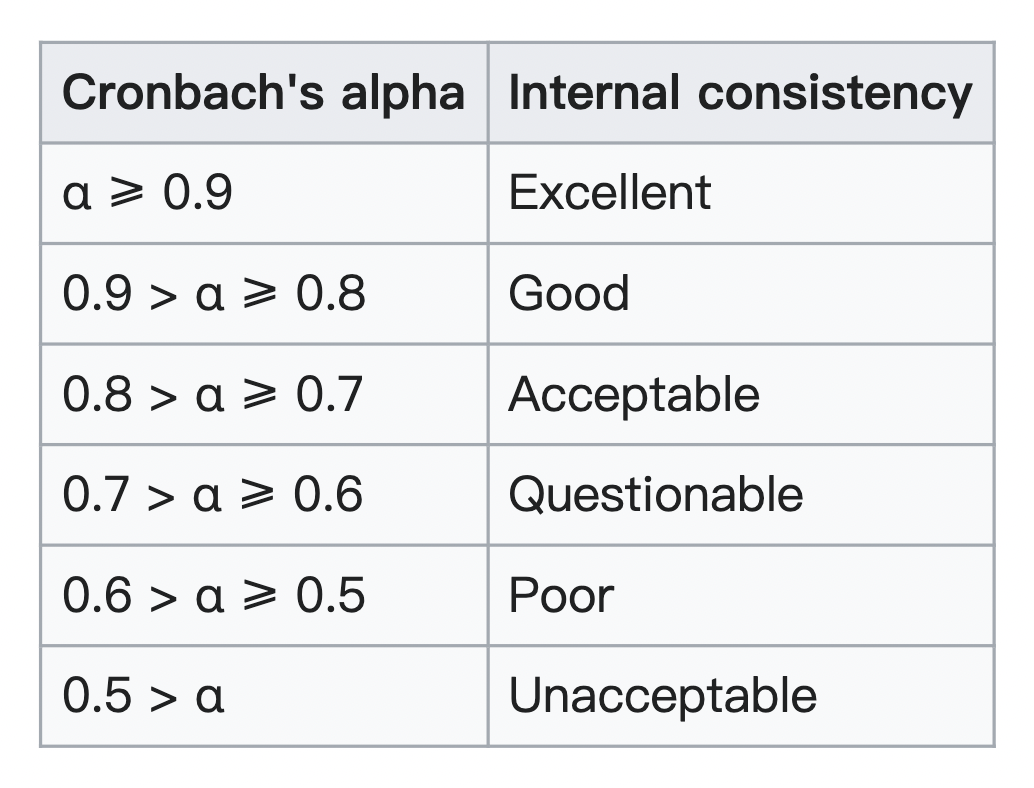
\includegraphics[width=0.5\linewidth]{Figure/Figure24.jpg}
  \centering
  \caption{Evaluation of score reliability coefficient test}
  \label{fig24}
\end{figure*}

\cleardoublepage
\subsection{SEM model 1}
\subsubsection{Path coefficient analysis for model 1}

SEM model 1 is shown in Figure~\ref{fig23}. The result of Regression Weights for Model 1 is shown in Table~\ref{table9}, and the result of Standard Regression Weights for Model 1 is shown in Table~\ref{table10}. From the result, we can find that Disaster Prevention Consciousness, Knowledge and Perception on earthquakes and Training Experience could show significant relationships with respondents' attitude toward Safety Tips, as p values are all less than 0.001. Also, Knowledge and Perception on earthquakes could show a positive relationship with respondents' attitude toward Safety Tips, as the estimated values are positive numbers (estimate value of Knowledge=3.066). While, Disaster Prevention Consciousness and Training Experience could show a negative relationship with respondents' attitude toward Safety Tips, as the estimate values are negative number (estimate value of Consciousness$=-2.191$; estimate value of Training Experience$=-0.433$;) 

\begin{figure*}[h]
  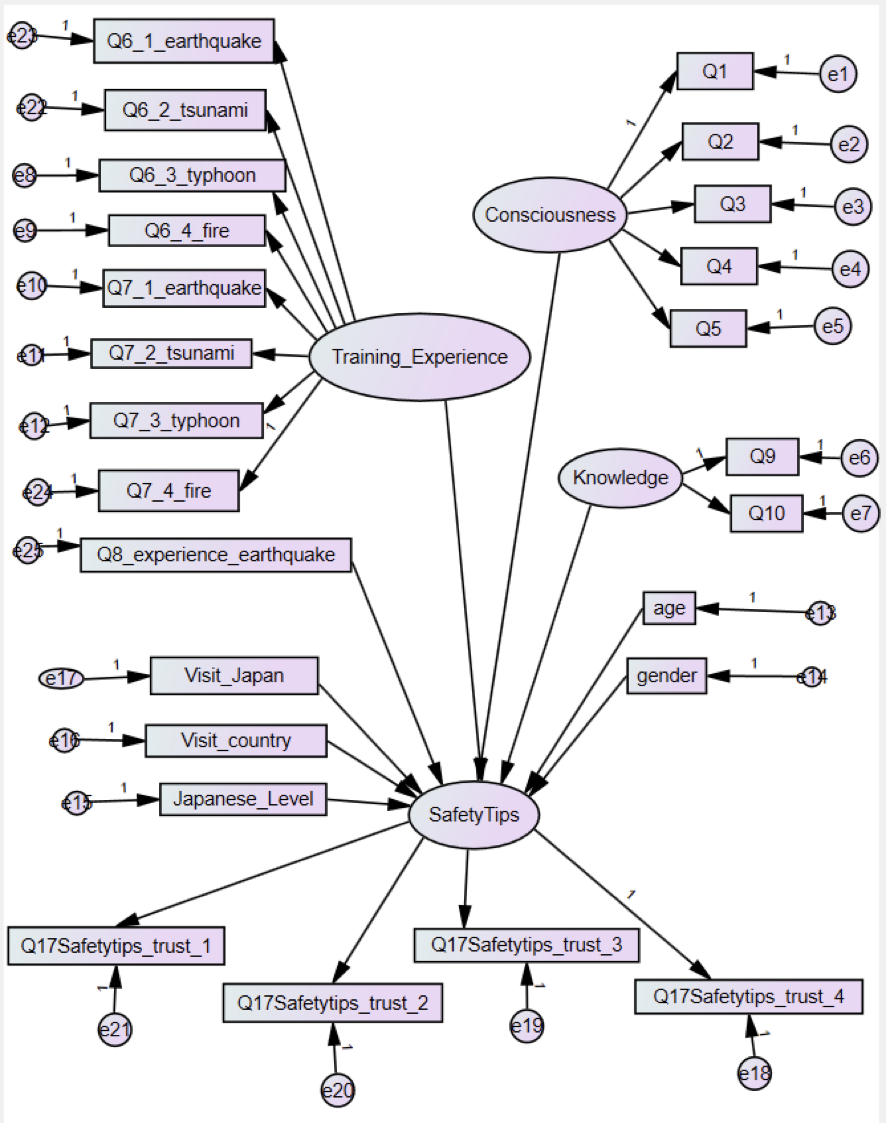
\includegraphics[width=0.5\linewidth]{Figure/Figure23.jpg}
  \centering
  \caption{SEM model 1}
  \label{fig23}
\end{figure*}

For four manifest variables age, number of visited Japan, number of visited countries, and Japanese level don't show significant relationships with respondents' attitudes toward Safety Tips, as p values are larger than 0.001 ($p_{age} =0.633$; $p_{visitedcountries} =0.628$; $p_{visitedJapan} =0.071$; $p_{JapaneseLevel} =0.265$). 


\begin{table}[h]
  \caption{Regression Weights of SEM model 1 }
  \label{table9}
  \centering
  \begin{tabular}{lcl|c|c}
 \hline
 \multicolumn{3}{c|}{Regression Weights} & Estimate & p-value \\
 \hline
SafetyTips              &$\longleftarrow$ & age                  & 0.013  & 0.633                \\
SafetyTips              &$\longleftarrow$ & Training\_Experience & -0.501 & ***                  \\
SafetyTips              &$\longleftarrow$ & Consciousness        & -2.785 & ***                  \\
SafetyTips              &$\longleftarrow$ & Knowledge            & 4.336  & ***                  \\
SafetyTips              &$\longleftarrow$ & VisitCountry         & -0.012 & 0.628                \\
SafetyTips              &$\longleftarrow$ & Japanese\_Level      & -0.049 & 0.265                \\
SafetyTips              &$\longleftarrow$ & VisitJapan           & 0.041  & 0.071                \\
Q1                      &$\longleftarrow$ & Consciousness        & 1      &  \\
Q2                      &$\longleftarrow$ & Consciousness        & 1.028  & ***                  \\
Q3                      &$\longleftarrow$ & Consciousness        & 1.029  & ***                  \\
Q4                      &$\longleftarrow$ & Consciousness        & 0.72   & ***                  \\
Q5                      &$\longleftarrow$ & Consciousness        & 0.157  & 0.052                \\
Q6\_1\_earthquake       &$\longleftarrow$ & Training\_Experience & 3.234  & ***                  \\
Q6\_2\_tsunami          &$\longleftarrow$ & Training\_Experience & 3.070   & ***                  \\
Q6\_3\_typhoon          &$\longleftarrow$ & Training\_Experience & 3.178  & ***                  \\
Q6\_4\_fire             &$\longleftarrow$ & Training\_Experience & 3.388  & ***                  \\
Q7\_1\_earthquake       &$\longleftarrow$ & Training\_Experience & 0.685  & ***                  \\
Q7\_2\_tsunami          &$\longleftarrow$ & Training\_Experience & 0.682  & ***                  \\
Q7\_3\_typhoon          &$\longleftarrow$ & Training\_Experience & 0.777  & ***                  \\
Q7\_4\_fire             &$\longleftarrow$ & Training\_Experience & 1      & \\
Q17Safetytips\_trust\_1 &$\longleftarrow$ & SafetyTips           & 1      &  \\
Q17Safetytips\_trust\_2 &$\longleftarrow$ & SafetyTips           & 0.826  & ***                  \\
Q17Safetytips\_trust\_3 &$\longleftarrow$ & SafetyTips           & 0.786  & ***                  \\
Q17Safetytips\_trust\_4 &$\longleftarrow$ & SafetyTips           & 0.688  & ***                 \\
 \hline
\multicolumn{5}{l}{*** means significant correlation at $p<0.001$.}
  \end{tabular}
\end{table}

\begin{table}[h]
  \caption{Standardized Regression Weights of SEM model 1 }
  \label{table10}
  \centering
  \begin{tabular}{lcl|c}
 \hline
 \multicolumn{3}{c|}{Standardized Regression Weights} & Estimate  \\
 \hline
SafetyTips              &$\longleftarrow$ & age                  & 0.015  \\
SafetyTips              &$\longleftarrow$ & Training\_Experience & -0.433 \\
SafetyTips              &$\longleftarrow$ & Consciousness        & -2.191 \\
SafetyTips              &$\longleftarrow$ & Knowledge            & 3.066  \\
SafetyTips              &$\longleftarrow$ & VisitCountry         & -0.016 \\
SafetyTips              &$\longleftarrow$ & Japanese\_Level      & -0.036 \\
SafetyTips              &$\longleftarrow$ & VisitJapan           & 0.058  \\
Q1                      &$\longleftarrow$ & Consciousness        & 0.809  \\
Q2                      &$\longleftarrow$ & Consciousness        & 0.843  \\
Q3                      &$\longleftarrow$ & Consciousness        & 0.855  \\
Q4                      &$\longleftarrow$ & Consciousness        & 0.576  \\
Q5                      &$\longleftarrow$ & Consciousness        & 0.092  \\
Q6\_1\_earthquake       &$\longleftarrow$ & Training\_Experience & 0.786  \\
Q6\_2\_tsunami          &$\longleftarrow$ & Training\_Experience & 0.838  \\
Q6\_3\_typhoon          &$\longleftarrow$ & Training\_Experience & 0.842  \\
Q6\_4\_fire             &$\longleftarrow$ & Training\_Experience & 0.758  \\
Q7\_1\_earthquake       &$\longleftarrow$ & Training\_Experience & 0.388  \\
Q7\_2\_tsunami          &$\longleftarrow$ & Training\_Experience & 0.489  \\
Q7\_3\_typhoon          &$\longleftarrow$ & Training\_Experience & 0.548  \\
Q7\_4\_fire             &$\longleftarrow$ & Training\_Experience & 0.566  \\
Q9                      &$\longleftarrow$ & Knowledge            & 0.785  \\
Q10                     &$\longleftarrow$ & Knowledge            & 0.804  \\
Q17Safetytips\_trust\_1 &$\longleftarrow$ & SafetyTips           & 0.816  \\
Q17Safetytips\_trust\_2 &$\longleftarrow$ & SafetyTips           & 0.822  \\
Q17Safetytips\_trust\_3 &$\longleftarrow$ & SafetyTips           & 0.834  \\
Q17Safetytips\_trust\_4 &$\longleftarrow$ & SafetyTips           & 0.717  \\
 \hline
  \end{tabular}
\end{table}

The result of the correlation relationship between Disaster Prevention Consciousness with Knowledge and Perception on earthquakes, also Knowledge and Perception on earthquakes with Training Experience was shown in Table~\ref{table13} and Table~\ref{table14}. The result confirmed that Disaster Prevention Consciousness with Knowledge and Perception on earthquakes, also Knowledge and Perception on earthquakes with Training Experience could both show a significant correlation, as p values are all less than 0.001. And both are positive correlations, as the estimated values are positive numbers (estimate the value of Consciousness and Knowledge=0.961; estimate the value of Training Experience and Knowledge=0.18;). Among them, Disaster Prevention Consciousness with Knowledge and Perception on earthquakes could show a higher correlation than Knowledge and Perception on earthquakes with Training Experience. 

\begin{table}[h]
  \caption{Covariances of SEM model 1}
  \label{table13}
  \centering
  \begin{tabular}{lcl|c|c}
  \hline
   \multicolumn{3}{c|}{Covariances} & Estimate & p-value \\
  \hline
  Consciousness & $\longleftrightarrow$ & Knowledge & 0.589 & *** \\
  Training\_Experience & $\longleftrightarrow$ & Knowledge & 0.121 & *** \\
  \hline
\multicolumn{5}{l}{*** means significant correlation at $p<0.001$.}
  \end{tabular}
\end{table}

\begin{table}[h]
  \caption{Correlations of SEM model 1}
  \label{table14}
  \centering
  \begin{tabular}{lcl|c}
  \hline
   \multicolumn{3}{c|}{Correlations} & Estimate \\
  \hline
  Consciousness & $\longleftrightarrow$ & Knowledge & 0.961 \\
  Training\_Experience & $\longleftrightarrow$ & Knowledge & 0.180 \\
  \hline
  \end{tabular}
\end{table}
\cleardoublepage
\subsubsection{Model Fit Test for SEM model 1}
The model fit result of Model 1 is shown in Table~\ref{table15}. From the results, CMIN/DF equals 8.352, an indicator that reflects model variability RMSEA equals 0.122, and an indicator that reflects model similarity CFI equals 0.738. Referring to some of the criteria mentioned in subsection~\ref{step6}, we can find that the model fit test of model 1 is not up to standard. Therefore, we need to modify model 1.

\begin{table}[h]
  \caption{Model fit test for SEM model 1}
  \label{table15}
  \centering 
  \begin{tabular}{|c|}
  \hline
  RMSEA = 0.122 \\
  CFI = 0.738 \\
  CMIN/DF = 8.352 \\
  \hline
  \end{tabular}
\end{table}

\subsubsection{Model adjustment and modification for model 1 }

We can get a better estimate of the true correlation by disattenuated the variables, and according to D. Streiner (2006)~\cite{Streiner2006BuildingAB}, two things happen when we add extra variables. First, the model's ability to account for more variance grows. Each new variable, on the other hand, enhances the error variance. As a result, the previous model will struggle to accommodate the additional data, which is a consequence of adding more variables to the model. 

We can see that Q6 1/2/3/4 and Q7 1/2/3/4 both have a significant relationship with Training Experience based on the results of Table~\ref{table9} Regression Weights. However, the estimated values of Q7 (Q7\_1=0.388; Q7\_2=0.489; Q7\_3=0.548; Q7\_4=0.566) are much lower than the estimated value of Q6 (Q6\_1=0.786; Q6\_2=0.838; Q6\_3=0.842; Q7\_4=0.758) , as seen in Table~\ref{table10} Standardized Regression Weights. This means that Q6 could be better than Q7 at expressing the latent variable Training Experience. The two manifest variables are similar in structure: Q6 is for the experience of a given event, and the total score is used as data, whereas Q7 is for the number of times. Because the similarity of the two variables causes a significant amount of inaccuracy in the expression of the latent variable, we'll delete Q7 and keep only Q6 as the manifest variable to express latent variable Training experience as a way to improve the model. 

Another point that could be improved in Q5. From the regression weights results presented in Table~\ref{table9}, we can find that the only manifest variable that does not significant is Q5, as the p-value of Q5 with Disaster Prevention Consciousness is $p=0.052>0.001$. This means that Q5 does not work well as a manifest variable for latent variables Disaster Prevention Consciousness. Therefore, model 2 will remove Q5 and use only Q1 to Q4 as the manifest variables.

Then, since the results show that manifest variables age, number of visited Japan, number of visited countries, and Japanese level have no significant relationship with Attitude toward Safety Tips, deleting these four variables could be also a way to improve the model. 
Based on the above three improvement ideas shown on the left side of Figure~\ref{fig25}, we construct Model 2 shown on the right side of Figure~\ref{fig25}.

\begin{figure*}[t]
  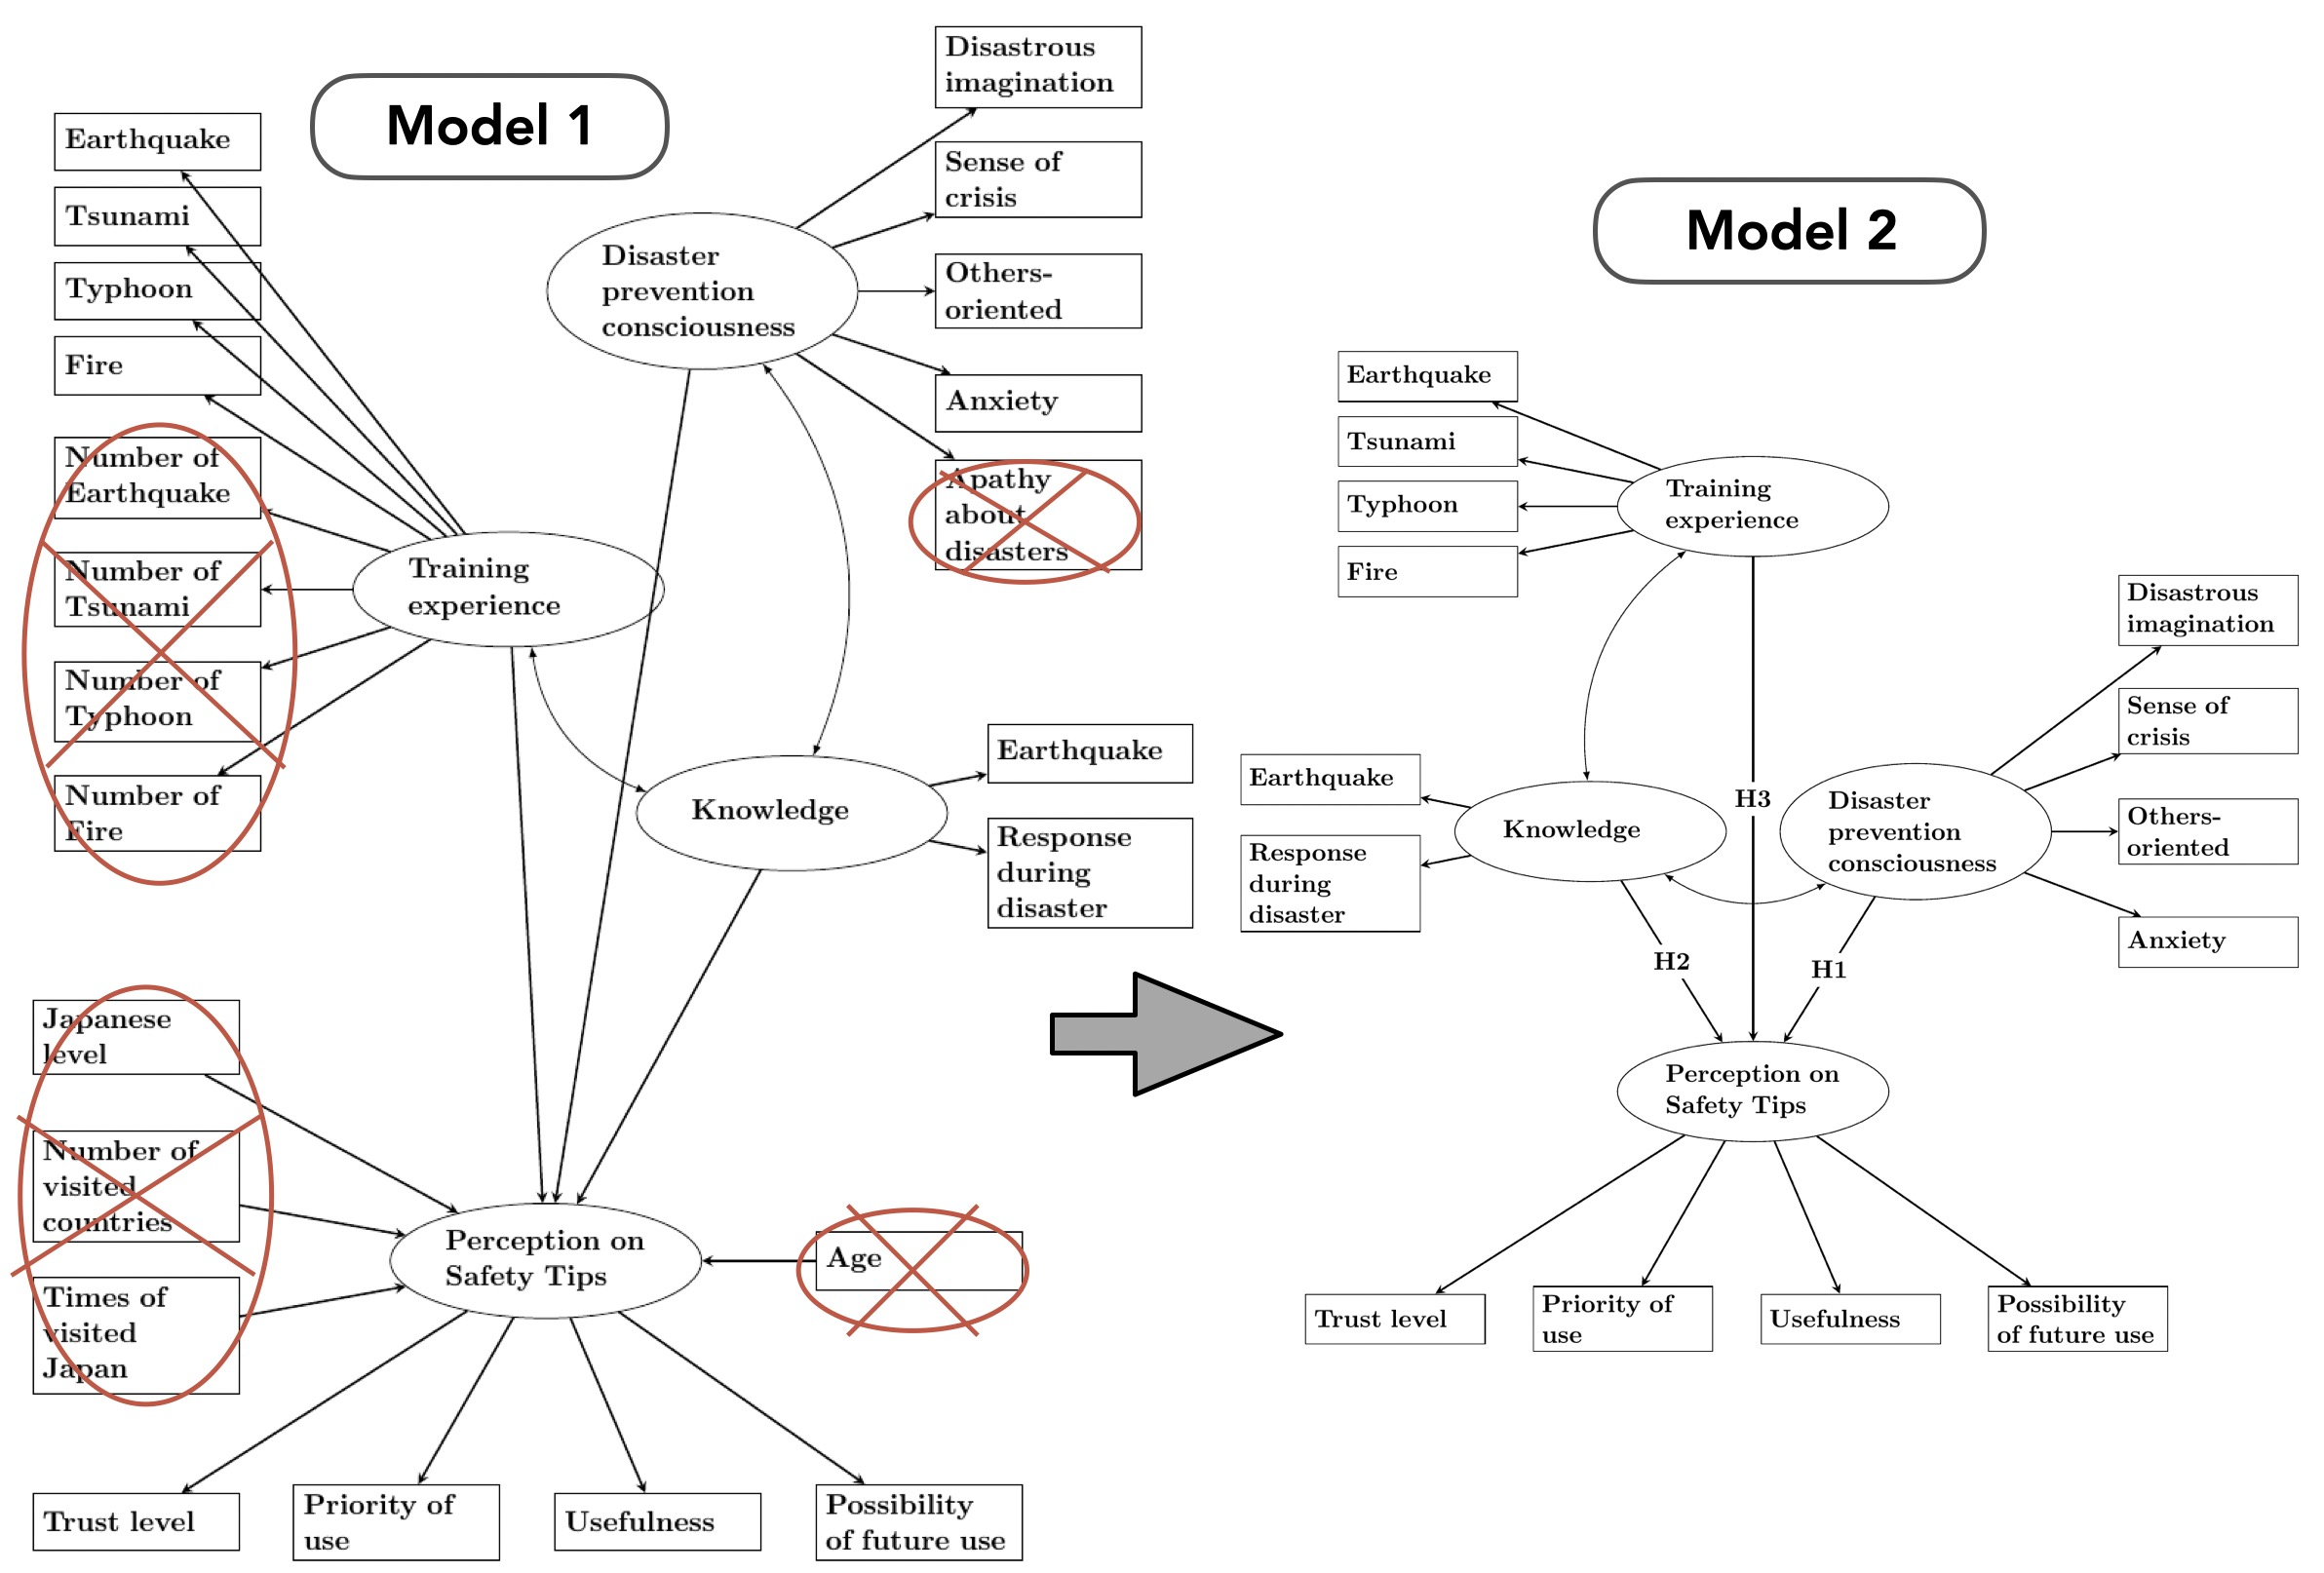
\includegraphics[width=\linewidth]{Figure/Figure25.png}
  \centering
  \caption[SEM model 2]{Left side: the diagram contains the improvement points made based on Model 1,Right side: Model 2}
  \label{fig25}
\end{figure*}




\subsection{SEM model 2}

\subsubsection{Model Fit Test for SEM model 2}
The model fit result of Model 2 is shown in Table~\ref{table16}. From the results, CMIN/DF equals 5.620, an indicator that reflects model variability RMSEA equals 0.097, an indicator that reflects model similarity CFI equals 0.925.

\begin{table}[h]
  \caption{Model fit test for SEM model 2}
  \label{table16}
  \centering 
  \begin{tabular}{|c|}
  \hline
  RMSEA = 0.097 \\
  CFI = 0.925 \\
  CMIN/DF = 5.620 \\
  \hline
  \end{tabular}
\end{table}

\subsubsection{Path coefficient analysis for model 2}
The result of Regression Weights for Model 2 is shown in Table~\ref{table11}, and the result of Standard Regression Weights for Model 2 is shown in Table~\ref{table12}. From the result, we can find that Disaster Prevention Consciousness and Knowledge and Perception on earthquakes could show significant relationships with respondents' attitude toward Safety Tips, as p values are both less than 0.001. But in model 2, Training Experience doesn't show significant relationships with respondents' attitude toward Safety Tips, as p values are larger than 0.001 ($p=0.002>0.001$). In other words, the regression weight for Training\_Experience in the prediction of SafetyTips is significantly different from zero at the 0.01 level (two-tailed). Then, from the result, we can find that Disaster Prevention Consciousness and Knowledge and Perception on earthquakes show opposite effects on respondents' attitude toward Safety Tips. Disaster Prevention Consciousness could show a negative relationship with respondents' attitude toward Safety Tips, as the estimated values are negative numbers (estimate value of Consciousness=-2.253). Knowledge and Perception on earthquakes could show a positive relationship with respondents' attitude toward Safety Tips, as the estimated values are positive numbers (estimate value of Knowledge=3.127). Also, we can find that all manifest variables could significantly express latent variables, as the p-value of all manifest variables could be less than 0.001. 

\begin{table}[t]
  \caption{Regression Weights of SEM model 2 }
  \label{table11}
  \centering
  \begin{tabular}{lcl|c|c}
 \hline
 \multicolumn{3}{c|}{Regression Weights} & Estimate & p-value \\
 \hline
SafetyTips              &$\longleftarrow$ & Training\_Experience & -0.147 & 0.002                \\
SafetyTips              &$\longleftarrow$ & Consciousness        & -2.876 & ***                  \\
SafetyTips              &$\longleftarrow$ & Knowledge            & 4.441  & ***                  \\
Q1                      &$\longleftarrow$ & Consciousness        & 1      &  \\
Q2                      &$\longleftarrow$ & Consciousness        & 1.027  & ***                  \\
Q3                      &$\longleftarrow$ & Consciousness        & 1.031  & ***                  \\
Q4                      &$\longleftarrow$ & Consciousness        & 0.715  & ***                  \\
Q6\_1\_earthquake       &$\longleftarrow$ & Training\_Experience & 1      &  \\
Q6\_2\_tsunami          &$\longleftarrow$ & Training\_Experience & 0.942  & ***                  \\
Q6\_3\_typhoon          &$\longleftarrow$ & Training\_Experience & 0.964  & ***                  \\
Q6\_4\_fire             &$\longleftarrow$ & Training\_Experience & 1.047  & ***                  \\
Q9                      &$\longleftarrow$ & Knowledge            & 1      &  \\
Q10                     &$\longleftarrow$ & Knowledge            & 1.003  & ***                  \\
Q17Safetytips\_trust\_1 &$\longleftarrow$ & SafetyTips           & 1      &  \\
Q17Safetytips\_trust\_2 &$\longleftarrow$ & SafetyTips           & 0.827  & ***                  \\
Q17Safetytips\_trust\_3 &$\longleftarrow$ & SafetyTips           & 0.786  & ***                  \\
Q17Safetytips\_trust\_4 &$\longleftarrow$ & SafetyTips           & 0.688  & ***                 \\
 \hline
\multicolumn{5}{l}{*** means significant correlation at $p<0.001$.}
  \end{tabular}
\end{table}

\begin{table}[h]
  \caption{Standardized Regression Weights of SEM model 2 }
  \label{table12}
  \centering
  \begin{tabular}{lcl|c}
 \hline
 \multicolumn{3}{c|}{Standardized Regression Weights} & Estimate  \\
 \hline
SafetyTips              &$\longleftarrow$ & Training\_Experience & -0.414 \\
SafetyTips              &$\longleftarrow$ & Consciousness        & -2.253 \\
SafetyTips              &$\longleftarrow$ & Knowledge            & 3.127  \\
Q1                      &$\longleftarrow$ & Consciousness        & 0.809  \\
Q2                      &$\longleftarrow$ & Consciousness        & 0.842  \\
Q3                      &$\longleftarrow$ & Consciousness        & 0.856  \\
Q4                      &$\longleftarrow$ & Consciousness        & 0.572  \\
Q6\_1\_earthquake       &$\longleftarrow$ & Training\_Experience & 0.792  \\
Q6\_2\_tsunami          &$\longleftarrow$ & Training\_Experience & 0.838  \\
Q6\_3\_typhoon          &$\longleftarrow$ & Training\_Experience & 0.833  \\
Q6\_4\_fire             &$\longleftarrow$ & Training\_Experience & 0.763  \\
Q9                      &$\longleftarrow$ & Knowledge            & 0.785  \\
Q10                     &$\longleftarrow$ & Knowledge            & 0.804  \\
Q17Safetytips\_trust\_1 &$\longleftarrow$ & SafetyTips           & 0.817  \\
Q17Safetytips\_trust\_2 &$\longleftarrow$ & SafetyTips           & 0.824  \\
Q17Safetytips\_trust\_3 &$\longleftarrow$ & SafetyTips           & 0.835  \\
Q17Safetytips\_trust\_4 &$\longleftarrow$ & SafetyTips           & 0.718  \\
 \hline
  \end{tabular}
\end{table}

The result of the correlation relationship between Disaster Prevention Consciousness with Knowledge and Perception on earthquakes, also Knowledge and Perception on earthquakes with Training Experience was shown in Table~\ref{table21} and Table~\ref{table22}. The result confirmed that Disaster Prevention Consciousness with Knowledge and Perception on earthquakes, also Knowledge and Perception on earthquakes with Training Experience could still both show a significant correlation, as p-values are all less than 0.001. And both are positive correlations, as the estimated values are positive numbers (estimate the value of Consciousness and Knowledge=0.963; estimate the value of Training Experience and Knowledge=0.175;). Among them, Knowledge and Perception on earthquakes with Disaster Prevention Consciousness could show a higher correlation than it with Training Experience, which is as same as in SEM model 1.

\begin{table}[h]
  \caption{Covariances of SEM model 2}
  \label{table21}
  \centering
  \begin{tabular}{lcl|c|c}
  \hline
   \multicolumn{3}{c|}{Covariances} & Estimate & p-value \\
  \hline
  Consciousness & $\longleftrightarrow$ & Knowledge & 0.590 & *** \\
  Training\_Experience & $\longleftrightarrow$ & Knowledge & 0.383 & *** \\
  \hline
\multicolumn{5}{l}{*** means significant correlation at $p<0.001$.}
  \end{tabular}
\end{table}

\begin{table}[h]
  \caption{Correlations of SEM model 2}
  \label{table22}
  \centering
  \begin{tabular}{lcl|c}
  \hline
   \multicolumn{3}{c|}{Correlations} & Estimate \\
  \hline
  Consciousness & $\longleftrightarrow$ & Knowledge & 0.963 \\
  Training\_Experience & $\longleftrightarrow$ & Knowledge & 0.175 \\
  \hline
  \end{tabular}
\end{table}
\cleardoublepage
\subsubsection{Confirmatory Factor Analysis (CFA)}
CFA include Construct Validity, Convergent Validity and Discriminant Validity, as explained in subsection~\ref{step5}.

\textbf{Construct Validity.} Referring to some of the criteria mentioned in subsection~\ref{step6}, from the model fit test From the model fit result shown in Table~\ref{table16}, we can find that the CFI estimate is satisfied in model 2, as a CFI of 0.9 or higher can be considered a good match~\cite{ref43,ref44}. And according to Schumacker and Lomax (2004)~\cite{ref39}, they suggested a more lenient fit around 5 or less, and the current CMIN/DF is near to 5, but a little bit higher than 5. Finally for RMSEA, according to Takahiro HOSHINO (2005)  (SEMres), as current RMSEA$=0.097<0.1$, the model shows a moderate fit. For measuring model Disaster Prevention Consciousness shown in Figure~\ref{fig31}, the results of Standardized Regression Weights (SRW) and Squared Multiple Correlations (SMC) are shown in Table~\ref{table24} and Table~\ref{table25}. From the results, we can find that all the SRW values are greater than 0.55, which means that SMC is greater than 0.30, satisfying the criteria mentioned in subsection~\ref{s7}, proving good. The model fit result of measuring model Disaster Prevention Consciousness is shown in Table~\ref{table26}. From the results, we can find that all model fit estimates are highly satisfying the criteria mentioned in subsection~\ref{step6}, as CMIN/DF equals 2.963, RMSEA equals 0.063, CFI equals 0.996. 


\begin{figure*}[t]
  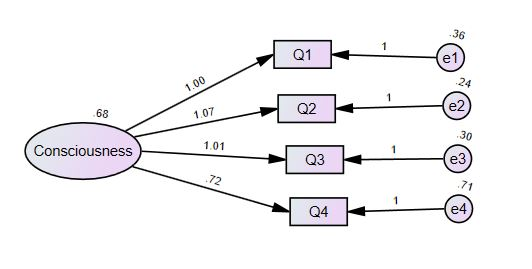
\includegraphics[width=0.5\linewidth]{Figure/figure31.JPG}
  \centering
  \caption{Measuring model of Consciousness}
  \label{fig31}
\end{figure*}

\begin{table}[h]
  \caption{Standardized Regression Weights for measuring model Consiousness}
  \label{table24}
  \centering
  \begin{tabular}{lcl|c}
  \hline
   \multicolumn{3}{c|}{Standardized Regression Weights} & Estimate \\
  \hline
  Q1 & $\longleftarrow$ & Consciousness & 0.807 \\
  Q2 & $\longleftarrow$ & Consciousness & 0.872 \\
  Q3 & $\longleftarrow$ & Consciousness & 0.835 \\
  Q4 & $\longleftarrow$ & Consciousness & 0.574 \\
  \hline
  \end{tabular}
\end{table}

\begin{table}[h]
  \caption{Squared Multiple Correlations for Consciousness}
  \label{table25}
  \centering
  \begin{tabular}{c|c}
  \hline
   Squared Multiple Correlations & Estimate \\
  \hline
  Q1  & 0.652 \\
  Q2  & 0.760 \\
  Q3  & 0.698 \\
  Q4  & 0.330 \\
  \hline
  \end{tabular}
\end{table}

\begin{table}[h]
  \caption{Model fit test for measuring model Consciousness}
  \label{table26}
  \centering 
  \begin{tabular}{|c|}
  \hline
  RMSEA = 0.063 \\
  CFI = 0.996 \\
  CMIN/DF = 2.963 \\
  \hline
  \end{tabular}
\end{table}

\textbf{Convergent Validity.} As mentioned in subsection~\ref{step5}, the commonly acceptable evaluation criterion of CR value in research should be above 0.7~\cite{ref32}. The result of the CR calculation is shown in Table~\ref{table35}. From the result, we can know that CR\_Consciousness$=0.857>0.7$; CR\_Training\_Experience$=0.882>0.7$; CR\_Knowledge$=1.001>0.7$; CR\_Attitude$=0.876>0.7$; This CR result can prove that the internal consistency of SEM is good. Also, according to Fornell and Larcker (1981)~\cite{ref31}, the commonly acceptable evaluation criterion of AVE value in research needs to be greater than 0.5. The result of the AVE calculation is also shown in Table~\ref{table35}. From the result, we can know that AVE\_Consciousness$=0.606>0.5$; AVE\_Training\_Experience$=0.651>0.5$; AVE\_Knowledge$=1.003>0.5$; AVE\_Attitude$=0.640>0.5$; This AVE result can prove that the explanatory power of the latent variables on the observed variables is good. In summary, the CR result and the AVE result show that SEM model 2 passed the Convergent Validity test. 

\begin{table}[h]
  \caption{Convergent Validity}
  \label{table35}
  \centering
  \begin{tabular}{lcl|cc|ccc}
  \hline
   & & & std.   & p-value           & SMC                  & CR                     & AVE                    \\
\hline
SafetyTips           & $\longleftarrow$       & Training\_Experience & -0.414 & 0.002                & \multicolumn{3}{l}{}    \\
SafetyTips           & $\longleftarrow$       & Consciousness        & -2.253 & ***                  & \multicolumn{3}{l}{} \\
SafetyTips           & $\longleftarrow$       & Knowledge            & 3.127  & ***                  & \multicolumn{3}{l}{}   \\
\hline
Q1                   & $\longleftarrow$       & Consciousness        & 0.809  &  & 0.654                & \multirow{4}{*}{0.857} & \multirow{4}{*}{0.606} \\
Q2                   & $\longleftarrow$       & Consciousness        & 0.842  & ***                  & 0.709                &                        &                        \\
Q3                   & $\longleftarrow$       & Consciousness        & 0.856  & ***                  & 0.733                &                        &                        \\
Q4                   & $\longleftarrow$       & Consciousness        & 0.572  & ***                  & 0.327                &                        &                        \\
\hline
Q6\_1                & $\longleftarrow$       & Training\_Experience & 0.792  &  & 0.627                & \multirow{4}{*}{0.882} & \multirow{4}{*}{0.651} \\
Q6\_2                & $\longleftarrow$       & Training\_Experience & 0.838  & ***                  & 0.702                &                        &                        \\
Q6\_3                & $\longleftarrow$       & Training\_Experience & 0.833  & ***                  & 0.694                &                        &                        \\
Q6\_4                & $\longleftarrow$       & Training\_Experience & 0.763  & ***                  & 0.582                &                        &                        \\
\hline
Q9                   & $\longleftarrow$       & Knowledge            & 0.785  &  & 0.616                & \multirow{2}{*}{1.001} & \multirow{2}{*}{1.003} \\
Q10                  & $\longleftarrow$       & Knowledge            & 0.804  & ***                  & 0.646                &                        &                        \\
\hline
Q17\_1               & $\longleftarrow$       & SafetyTips           & 0.817  &  & 0.667                & \multirow{4}{*}{0.876} & \multirow{4}{*}{0.64}  \\
Q17\_2               & $\longleftarrow$       & SafetyTips           & 0.824  & ***                  & 0.679                &                        &                        \\
Q17\_3               & $\longleftarrow$       & SafetyTips           & 0.835  & ***                  & 0.697                &                        &                        \\
Q17\_4               & $\longleftarrow$       & SafetyTips           & 0.718  & ***                  & 0.516                &                        &                       \\
  \hline
\multicolumn{5}{l}{*** means significant correlation at $p<0.001$.}
  \end{tabular}
\end{table}




\textbf{Discriminant Validity.} As mentioned in subsection~\ref{step5}, this study decided to use AVE to compare whether the mean AVE of two latent variables was greater than the squared correlation coefficient of the two latent variables~\cite{ref31} as the method of doing a Discriminant Validity test. Here, for operational convenience, we compare the positive square root of the AVE value of the latent variables and the correlation coefficient of the latent variables. The result of the calculation is shown in Table~\ref{table36}. From the result, we can find that SQRT\_AVE\_Knowledge=1.001, this value is larger than the correlation coefficient of Knowledge with the other three latent variables. Then, SQRT\_AVE\_Consciousness=0.778, this value is larger than the correlation coefficient of Consciousness with Training experience and Attitude, but it is smaller than the correlation coefficient of Consciousness with Knowledge. Next is SQRT\_AVE\_Training\_experience=0.807, this value is larger than the correlation coefficient of Training experience with the other three latent variables. Finally, SQRT\_AVE\_Attitude=0.800, this value is larger than the correlation coefficient of Attitude with Training experience and Consciousness, but it is smaller than the correlation coefficient of Attitude with Knowledge. As Discriminant Validity is to see whether the differentiation between different dimensions and between topics meets the standard. All the problematic items appear on top of Knowledge and Perception on earthquakes, which I think is due to the fact that there are only two manifest variables of this latent variable, which are not enough to accurately represent Knowledge and Perception on earthquakes on the SEM model. This is also a reason that the model fitness is affected in this study due to the limitation of survey data. But in general, the Discriminant Validity of this SEM model 2 could still be fine.

\begin{table}[h]
  \caption{Discriminant Validity }
  \label{table36}
  \centering
\makebox[1 \textwidth][c]{  
\resizebox{1\textwidth}{!}{
\begin{tabular}{c|ccccc}
\hline
     & AVE   & Knowledge                             & Consciousness                         & Training\_Experience                  & \multicolumn{1}{c}{SafetyTips}                          \\
\hline
Knowledge            & 1.003 & \textcolor{red}{\textbf{1.001}} & \multicolumn{1}{l}{}                  & \multicolumn{1}{l}{}                  &                                                         \\
Consciousness        & 0.606 & 0.963***                              & \textcolor{red}{\textbf{0.778}} & \multicolumn{1}{l}{}                  &                                                         \\
Training\_Experience & 0.651 & 0.175***                              & 0                                     & \textcolor{red}{\textbf{0.807}} &                                                         \\
SafetyTips           & 0.64  & 0.885***                              & 0.760***                              & 0.133                                     & \textcolor{red}{\textbf{0.8}}\\
  \hline
\multicolumn{5}{l}{*** means significant correlation at $p<0.001$.}
  \end{tabular}
}}
\end{table}

\subsubsection{Hypothesis testing and conclusion analysis}
\begin{itemize}
\item[\textbf{H1}] Disaster Prevention Consciousness has a positive impact on respondents' attitudes toward Safety Tips.
\item[\textbf{$\longrightarrow$}] This Hypothesis is inconsistent with hypothesis H1. Disaster Prevention Consciousness has a negative impact on respondents' attitudes toward Safety Tips.
\item[\textbf{H2}] Knowledge and Perception of earthquakes have a positive impact on respondents' attitudes toward Safety Tips.
\item[\textbf{$\longrightarrow$}] This Hypothesis is consistent with hypothesis H2. 
\item[\textbf{H3}] Training Experience has a positive impact on respondents' attitudes toward Safety Tips.
\item[\textbf{$\longrightarrow$}] This Hypothesis is inconsistent with hypothesis H3. Training Experience does not have a significant impact on respondents' attitudes toward Safety Tips.
\end{itemize}

\subsubsection{Interpretation}
The following sections will explain how to interpret the aforesaid results. 

Disaster Prevention Consciousness has a negative impact on respondents' attitudes toward Safety Tips: for all those who have a higher consciousness about the disaster, it means they have a higher disaster imagination, sense, and are more likely to feel anxiety about the disaster, and they are more likely to come into contact with people, so they would prefer a more direct way to evacuate rather than seeking information, which makes their attitude toward safety tips could be negative.
Knowledge and Perception of earthquakes have a positive impact on respondents' attitudes toward Safety Tips: people with richer knowledge, are relatively more aware of the importance of information seeking for evacuation. Therefore, their attitudes towards Safety Tips could be better than others.

Training Experience does not have a significant impact on respondents' attitudes toward Safety Tips: respondents with more earthquake or disaster training experience should be more knowledgeable with earthquake evacuation ways, therefore their attitude toward safety suggestions may be negative as well. 




\section{Results for Objective 3}

\subsection{Selected Score and Selected Rate}
The result of the Selected score and the Selected rate is shown in \crefrange{table17}{table20}. From the result, we can find that there are some differences between foreign visitors and Japanese in scenarios 1 and 3, which could show that when the internet and telephone are available, people tend to have various behaviors. By checking the Selected Rate, we can find that evacuation behaviors are more used than information-seeking behaviors. And among the evacuation behaviors, 'Moving according to evacuation guidance' could be used most. This indicates that, regardless of the order factor, 'Moving according to evacuation guidance' is the most favored option. In addition, people are more likely to heed evacuation instructions if they are in the area of such recommendations.  By checking the Selected Score, we can find that evacuation behaviors always happen before information-seeking behaviors. And among the evacuation behaviors, 'Observe the surroundings' could have happened first. This is compounded by the fact that many people's first instinct in the event of a disaster is to observe others. Not only might they receive some evacuation suggestions, but keeping the same pace as others will make people feel more at ease psychologically. 

Some lower used information-seeking behaviors during a disaster are 'Gather Information by calling out to Japanese people nearby', 'Contact staff at tourist Information centers to collect Information', 'Contact public transport staff to collect Information'. As a result, in the case of Internet\&Phone available, people do not choose to acquire information through methods that require verbal conversation, and instead prefer to obtain it on their own. On the other hand, because people can only obtain information through the verbal conversation when the Internet and phone are unavailable, their method of obtaining information depends on the scenario they are in. When people are in a tourist area, they usually ask Japanese people around them for information, and not many people choose the other three options of contacting staff at different spots. However, when people are moving by transportation, people still ask Japanese people around them for information, while contacting staff from public transportation is also a popular option. The lowest used evacuation behavior during a disaster is 'Stay at your current location. This is understandable after all, few people will just stay put and do nothing in the face of a disaster. It is important to note here that this result does not mean that everyone will necessarily do something to leave the place where it happened, but that people's priority evacuation behavior is less likely to be to stay where they are. People will, in most situations, choose to remain where they are after gathering information and following evacuation instructions. This section does not cover such circumstances.

%%%%%%%%%%%%%%%%%%%%%%%%%%
%\iffalse
\begin{table}[h]
  \caption[Result of Selected score and Selected rate in Scenario 1]{Result of Selected score and Selected rate in Scenario 1(No.: number of  selection, FV: Foreign Vistors, J: Japanese)}
  \label{table17}
  \centering 
  \begin{tabular}{cl|ccc|ccc}
                &   & \multicolumn{3}{c}{Selected Rate (\%)} & \multicolumn{3}{c}{Selected Score} \\
      No.     & \multicolumn{1}{c|}{Description} & All & FV & J & All & FV & J \\
 \hline
  1             & \begin{tabular}{l}Collect Information on the official websites\\of Japanese government agencies\end{tabular} & 31.6 &30.2 & 38.7 & 2.9 & 2.9 & 3.0 \\
  2             & \begin{tabular}{l}Collect Information with the disaster\\prevention app on your smartphone\end{tabular} & 27.9 & 25.4 & 40.7 & 2.9 & 2.8 & 3.2 \\
  3             & \begin{tabular}{l}Collect Information on news sites and\\disaster prevention portal sites\end{tabular} & 26.8 & 23.4 & 43.7 & 2.8 & 2.7 & 3.2 \\
  4             & \begin{tabular}{l}Collect Information on SNS\\(Twitter, Facebook, LINE, etc.)\end{tabular} & 19.9 & 18.2 & 28.7 & 2.8 & 2.7 & 3.0 \\
  5             & \begin{tabular}{l}Call the embassy of your country\\to collect Information\end{tabular} & 25.2 & 30.3 & N/A & 2.7 & 2.7 & N/A \\
  6             & \begin{tabular}{l}Collect Information from TV and radio\end{tabular} & 24.9 & 20.9 & 44.7 & 3.0 & 2.8 & 3.4 \\
  7             & \begin{tabular}{l}Check maps and digital signage to\\collect Information\end{tabular} & 14.4 & 15.0 & 11.7 & 2.8 & 2.8 & 2.9 \\
  8             & \begin{tabular}{l}Gather Information by calling out to\\Japanese people nearby\end{tabular} & 18.7 & 19.0 & 17.3 & 2.7 & 2.8 & 2.3 \\
  9             & \begin{tabular}{l}Contact staff at tourist Information\\centers to collect Information\end{tabular} & 16.0 & 18.3 & 4.3 & 2.9 & 2.9 & 2.3 \\
 10            & \begin{tabular}{l}Contact the hotel staff to collect\\Information\end{tabular} & 15.8 & 17.0 & 10.0 & 2.8 & 2.8 & 2.8 \\
 11            & \begin{tabular}{l}Contact public transport staff to\\collect Information\end{tabular} & 13.9 & 13.7 & 14.7 & 2.5 & 2.6 & 2.4 \\
 12            & \begin{tabular}{l}Stay at your current location\end{tabular} & 16.6 & 17.5 & 12.0 & 3.4 & 3.4 & 3.5 \\
 13            & \begin{tabular}{l}Secure necessary supplies\\(food, drink, etc.)\end{tabular}  & 32.9 & 33.0 & 32.3 & 3.0 & 3.1 & 2.8 \\
 14            & \begin{tabular}{l}Move to an open space such as a\\nearby park\end{tabular} & 39.7 & 41.8 & 29.0 & 3.3 & 3.3 & 3.0 \\
 15            & \begin{tabular}{l}Move according to evacuation\\guidance\end{tabular} & 53.7 & 54.9 & 47.7 & 3.4 & 3.5 & 3.2 \\
 16            & \begin{tabular}{l}Move to the evacuation center on\\your own\end{tabular} & 26.8 & 27.1 & 25.0 & 3.1 & 3.1 & 3.0 \\
 17            & \begin{tabular}{l}Move in sync with the movements\\of people around you\end{tabular} & 28.3 & 29.2 & 24.0 & 2.8 & 2.9 & 2.6 \\
 18            & \begin{tabular}{l}Observe the surroundings because\\you don't know what to do\end{tabular} & 45.2 & 44.7 & 48.0 & 3.6 & 3.6 & 3.4 \\
\hline
  \end{tabular}
\end{table}


\begin{table}[h]
  \caption[Result of Selected score and Selected rate in Scenario 2]{Result of Selected score and Selected rate in Scenario 2(No.: number of  selection, FV: Foreign Vistors, J: Japanese)}
  \label{table18}
  \centering 
  \begin{tabular}{cl|ccc|ccc}
                &   & \multicolumn{3}{c}{Selected Rate (\%)} & \multicolumn{3}{c}{Selected Score} \\
      No.     & \multicolumn{1}{c|}{Description} & All & FV & J & All & FV & J \\
 \hline
  8             & \begin{tabular}{l}Gather Information by calling out to\\Japanese people nearby\end{tabular} & 41.1 & 40.5 & 44.0 & 2.8 & 2.8 & 2.9 \\
  9             & \begin{tabular}{l}Contact staff at tourist Information\\centers to collect Information\end{tabular} & 33.8 & 36.8 & 18.7 & 2.7 & 2.7 & 2.4 \\
 10            & \begin{tabular}{l}Contact the hotel staff to collect\\Information\end{tabular} & 33.0 & 34.3 & 26.7 & 2.9 & 2.8 & 3.0 \\
 11            & \begin{tabular}{l}Contact public transport staff to\\collect Information\end{tabular} & 29.8 & 29.3 & 32.7 & 2.7 & 2.6 & 2.8 \\
 12            & \begin{tabular}{l}Stay at your current location\end{tabular} & 23.9 & 24.7 & 20.0 & 3.0 & 3.0 & 3.0 \\
 13            & \begin{tabular}{l}Secure necessary supplies\\(food, drink, etc.)\end{tabular}  & 44.5 & 44.4 & 45.0 & 2.9 & 2.9 & 3.0 \\
 14            & \begin{tabular}{l}Move to an open space such as a\\nearby park\end{tabular} & 52.5 & 54.5 & 44.7 & 3.2 & 3.2 & 3.1 \\
 15            & \begin{tabular}{l}Move according to evacuation\\guidance\end{tabular} & 66.6 & 65.9 & 70.0 & 3.4 & 3.4 & 3.5 \\
 16            & \begin{tabular}{l}Move to the evacuation center on\\your own\end{tabular} & 39.3 & 37.9 & 46.3 & 2.9 & 2.9 & 2.7 \\
 17            & \begin{tabular}{l}Move in sync with the movements\\of people around you\end{tabular} & 46.5 & 47.3 & 42.7 & 2.9 & 3.0 & 2.8 \\
 18            & \begin{tabular}{l}Observe the surroundings because\\you don't know what to do\end{tabular} & 61.6 & 60.7 & 66.0 & 3.6 & 3.5 & 3.8 \\
\hline
  \end{tabular}
\end{table}



\begin{table}[h]
  \caption[Result of Selected score and Selected rate in Scenario 3]{Result of Selected score and Selected rate in Scenario 3(No.: number of  selection, FV: Foreign Vistors, J: Japanese)}
  \label{table19}
  \centering 
  \begin{tabular}{cl|ccc|ccc}
                &   & \multicolumn{3}{c}{Selected Rate (\%)} & \multicolumn{3}{c}{Selected Score} \\
      No.     & \multicolumn{1}{c|}{Description} & All & FV & J & All & FV & J \\
 \hline
  1             & \begin{tabular}{l}Collect Information on the official websites\\of Japanese government agencies\end{tabular} & 29.1 & 28.6 & 31.1 & 3.0 & 3.0 & 3.0 \\
  2             & \begin{tabular}{l}Collect Information with the disaster\\prevention app on your smartphone\end{tabular} & 29.4 & 27.1 & 41.0 & 3.0 & 2.9 & 3.2 \\
  3             & \begin{tabular}{l}Collect Information on news sites and\\disaster prevention portal sites\end{tabular} & 27.6 & 24.5 & 43.0 & 2.8 & 2.7 & 3.2 \\
  4             & \begin{tabular}{l}Collect Information on SNS\\(Twitter, Facebook, LINE, etc.)\end{tabular} & 24.6 & 22.7 & 34.3 & 2.8 & 2.7 & 3.0 \\
  5             & \begin{tabular}{l}Call the embassy of your country\\to collect Information\end{tabular} & 24.2 & 29.0 & N/A & 2.9 & 2.9 & N/A \\
  6             & \begin{tabular}{l}Collect Information from TV and radio\end{tabular} & 22.4 & 19.3 & 37.7 & 2.9 & 2.8 & 3.0 \\
  7             & \begin{tabular}{l}Check maps and digital signage to\\collect Information\end{tabular} & 15.7 & 16.2 & 13.3 & 2.9 & 2.9 & 2.9 \\
  8             & \begin{tabular}{l}Gather Information by calling out to\\Japanese people nearby\end{tabular} & 20.7 & 21.1 & 18.3 & 2.7 & 2.7 & 2.7 \\
  9             & \begin{tabular}{l}Contact staff at tourist Information\\centers to collect Information\end{tabular} & 16.8 & 18.8 & 7.0 & 2.7 & 2.7 & 2.7 \\
 10            & \begin{tabular}{l}Contact the hotel staff to collect\\Information\end{tabular} & 15.4 & 17.1 & 7.0 & 2.8 & 2.8 & 2.9 \\
 11            & \begin{tabular}{l}Contact public transport staff to\\collect Information\end{tabular} & 23.9 & 22.6 & 30.7 & 3.0 & 3.0 & 3.1 \\
 12            & \begin{tabular}{l}Stay at your current location\end{tabular} & 13.7 & 14.3 & 10.3 & 3.6 & 3.7 & 2.9 \\
 13            & \begin{tabular}{l}Secure necessary supplies\\(food, drink, etc.)\end{tabular}  & 27.8 & 28.3 & 25.3 & 3.0 & 3.0 & 2.9 \\
 14            & \begin{tabular}{l}Move to an open space such as a\\nearby park\end{tabular} & 34.6 & 37.6 & 19.3 & 3.2 & 3.2 & 2.9 \\
 15            & \begin{tabular}{l}Move according to evacuation\\guidance\end{tabular} & 50.7 & 50.9 & 50.0 & 3.4 & 3.4 & 3.2 \\
 16            & \begin{tabular}{l}Move to the evacuation center on\\your own\end{tabular} & 26.6 & 27.9 & 20.3 & 2.9 & 2.9 & 2.8 \\
 17            & \begin{tabular}{l}Move in sync with the movements\\of people around you\end{tabular} & 32.4 & 33.6 & 26.7 & 2.9 & 2.9 & 2.8 \\
 18            & \begin{tabular}{l}Observe the surroundings because\\you don't know what to do\end{tabular} & 41.1 & 40.8 & 42.7 & 3.7 & 3.7 & 3.5 \\
\hline
  \end{tabular}
\end{table}


\begin{table}[h]
  \caption[Result of Selected score and Selected rate in Scenario 4]{Result of Selected score and Selected rate in Scenario 4(No.: number of  selection, FV: Foreign Vistors, J: Japanese)}
  \label{table20}
  \centering 
  \begin{tabular}{cl|ccc|ccc}
                &   & \multicolumn{3}{c}{Selected Rate (\%)} & \multicolumn{3}{c}{Selected Score} \\
      No.     & \multicolumn{1}{c|}{Description} & All & FV & J & All & FV & J \\
 \hline
  8             & \begin{tabular}{l}Gather Information by calling out to\\Japanese people nearby\end{tabular} & 42.3 & 43.4 & 37.0 & 2.8 & 2.8 & 2.8 \\
  9             & \begin{tabular}{l}Contact staff at tourist Information\\centers to collect Information\end{tabular} & 29.2 & 32.1 & 14.7 & 2.7 & 2.7 & 2.7 \\
 10            & \begin{tabular}{l}Contact the hotel staff to collect\\Information\end{tabular} & 27.2 & 29.5 & 15.7 & 2.9 & 2.9 & 2.8 \\
 11            & \begin{tabular}{l}Contact public transport staff to\\collect Information\end{tabular} & 40.9 & 39.4 & 48.3 & 3.1 & 3.0 & 3.4 \\
 12            & \begin{tabular}{l}Stay at your current location\end{tabular} & 24.3 & 24.8 & 21.7 & 3.1 & 3.2 & 3.0 \\
 13            & \begin{tabular}{l}Secure necessary supplies\\(food, drink, etc.)\end{tabular}  & 39.1 & 39.2 & 38.3 & 2.8 & 2.9 & 2.8 \\
 14            & \begin{tabular}{l}Move to an open space such as a\\nearby park\end{tabular} & 49.8 & 52.2 & 37.7 & 3.0 & 3.0 & 2.6 \\
 15            & \begin{tabular}{l}Move according to evacuation\\guidance\end{tabular} & 67.7 & 66.2 & 75.0 & 3.5 & 3.4 & 3.6 \\
 16            & \begin{tabular}{l}Move to the evacuation center on\\your own\end{tabular} & 41.1 & 40.9 & 42.0 & 2.8 & 2.8 & 2.5 \\
 17            & \begin{tabular}{l}Move in sync with the movements\\of people around you\end{tabular} & 50.6 & 50.9 & 49.0 & 2.9 & 3.0 & 2.8 \\
 18            & \begin{tabular}{l}Observe the surroundings because\\you don't know what to do\end{tabular} & 59.2 & 57.5 & 67.7 & 3.5 & 3.5 & 3.6 \\
\hline
  \end{tabular}
\end{table}
%\fi
\cleardoublepage
\subsection{Sankey Diagram}

Figure~\ref{fig26} depicts the Sankey Diagram for foreign visitors in scenarios 1 to 4, whereas Figure~\ref{fig27} depicts the Sankey Diagram for Japanese visitors in scenarios 1 to 4. Figure~\ref{fig28} shows a summary of the Sankey Diagram data, with blue denoting the action with the highest value. 

%%%%%%%%%%%%%%%%%%%%%%%%%%
%\iffalse
\begin{figure*}[h]
  \begin{subfigure}{0.5\textwidth}
    \centering
    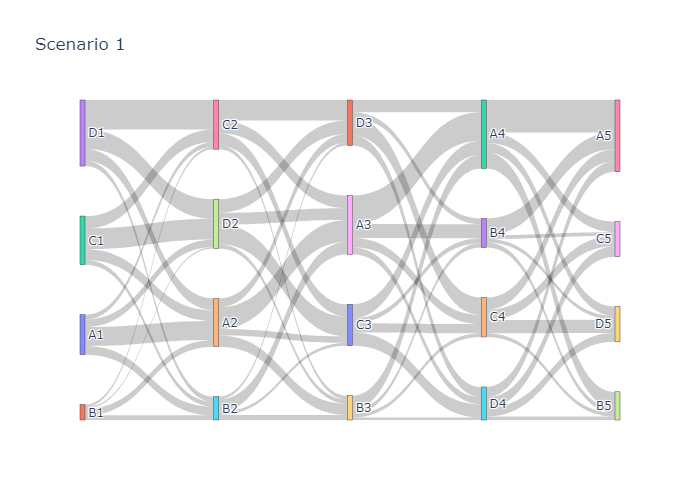
\includegraphics[width=\textwidth]{Figure/Figure26a.jpg}
    \caption{In scenario 1}
    \label{fig26a}
  \end{subfigure}
  \begin{subfigure}{0.5\textwidth}
    \centering
    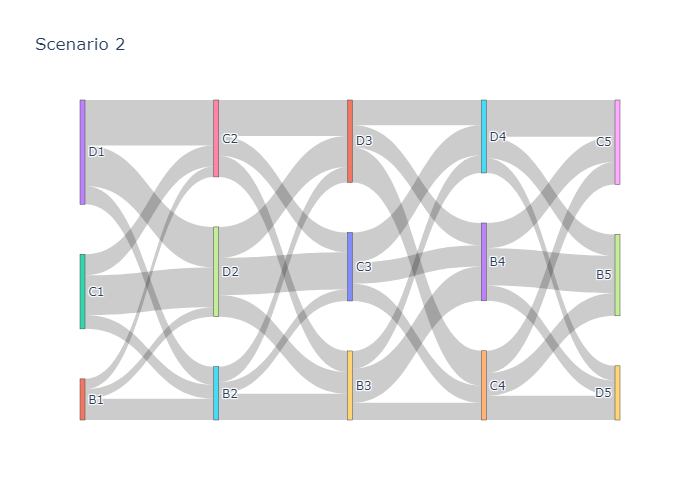
\includegraphics[width=\linewidth]{Figure/Figure26b.jpg}
    \caption{In scenario 2}
    \label{fig26b}
  \end{subfigure}
  \begin{subfigure}{0.5\textwidth}
    \centering
    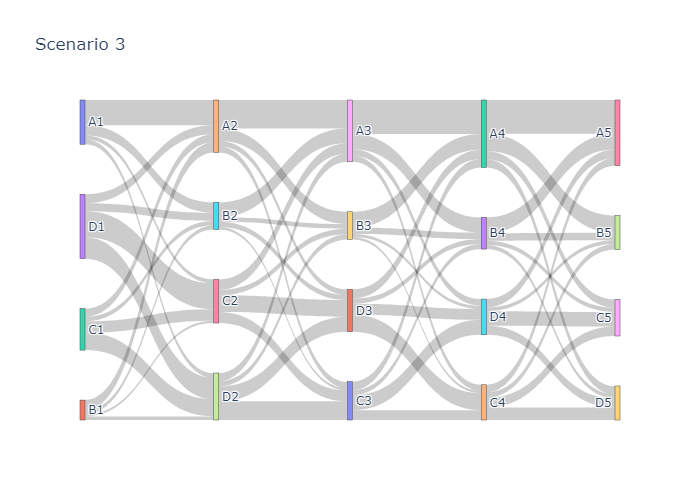
\includegraphics[width=\linewidth]{Figure/Figure26c.jpg}
    \caption{In scenario 3}
    \label{fig26c}
  \end{subfigure}
  \begin{subfigure}{0.5\textwidth}
    \centering
    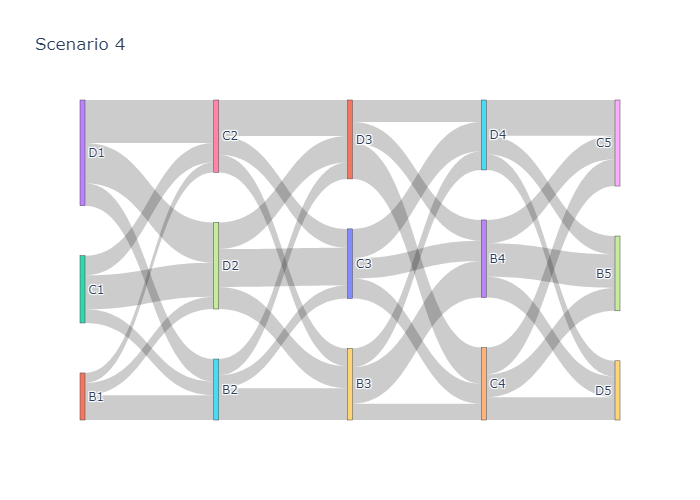
\includegraphics[width=\linewidth]{Figure/Figure26d.jpg}
    \caption{In scenario 4}
    \label{fig26d}
  \end{subfigure}
  \caption{Sankey diagram of foreign visitors }
  \label{fig26}
\end{figure*}

\begin{figure*}[h]
  \begin{subfigure}{0.5\textwidth}
    \centering
    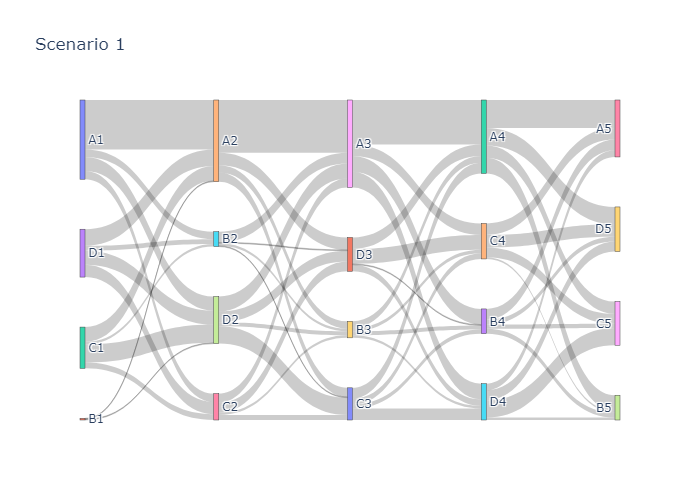
\includegraphics[width=\textwidth]{Figure/Figure27a.jpg}
    \caption{In scenario 1}
    \label{fig27a}
  \end{subfigure}
  \begin{subfigure}{0.5\textwidth}
    \centering
    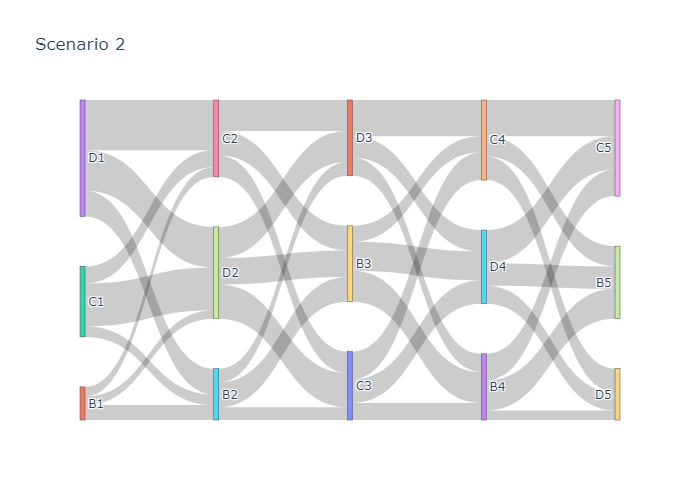
\includegraphics[width=\linewidth]{Figure/Figure27b.jpg}
    \caption{In scenario 2}
    \label{fig27b}
  \end{subfigure}
  \begin{subfigure}{0.5\textwidth}
    \centering
    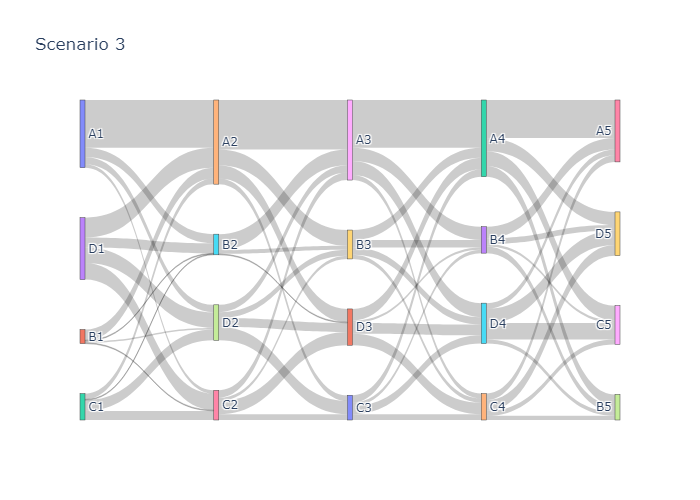
\includegraphics[width=\linewidth]{Figure/Figure27c.jpg}
    \caption{In scenario 3}
    \label{fig27c}
  \end{subfigure}
  \begin{subfigure}{0.5\textwidth}
    \centering
    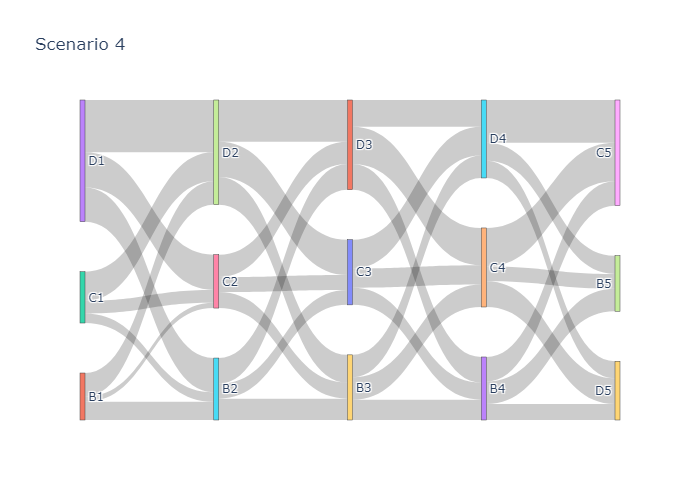
\includegraphics[width=\linewidth]{Figure/Figure27d.jpg}
    \caption{In scenario 4}
    \label{fig27d}
  \end{subfigure}
  \caption{Sankey diagram of Japanese }
  \label{fig27}
\end{figure*}

\begin{figure*}[h]
  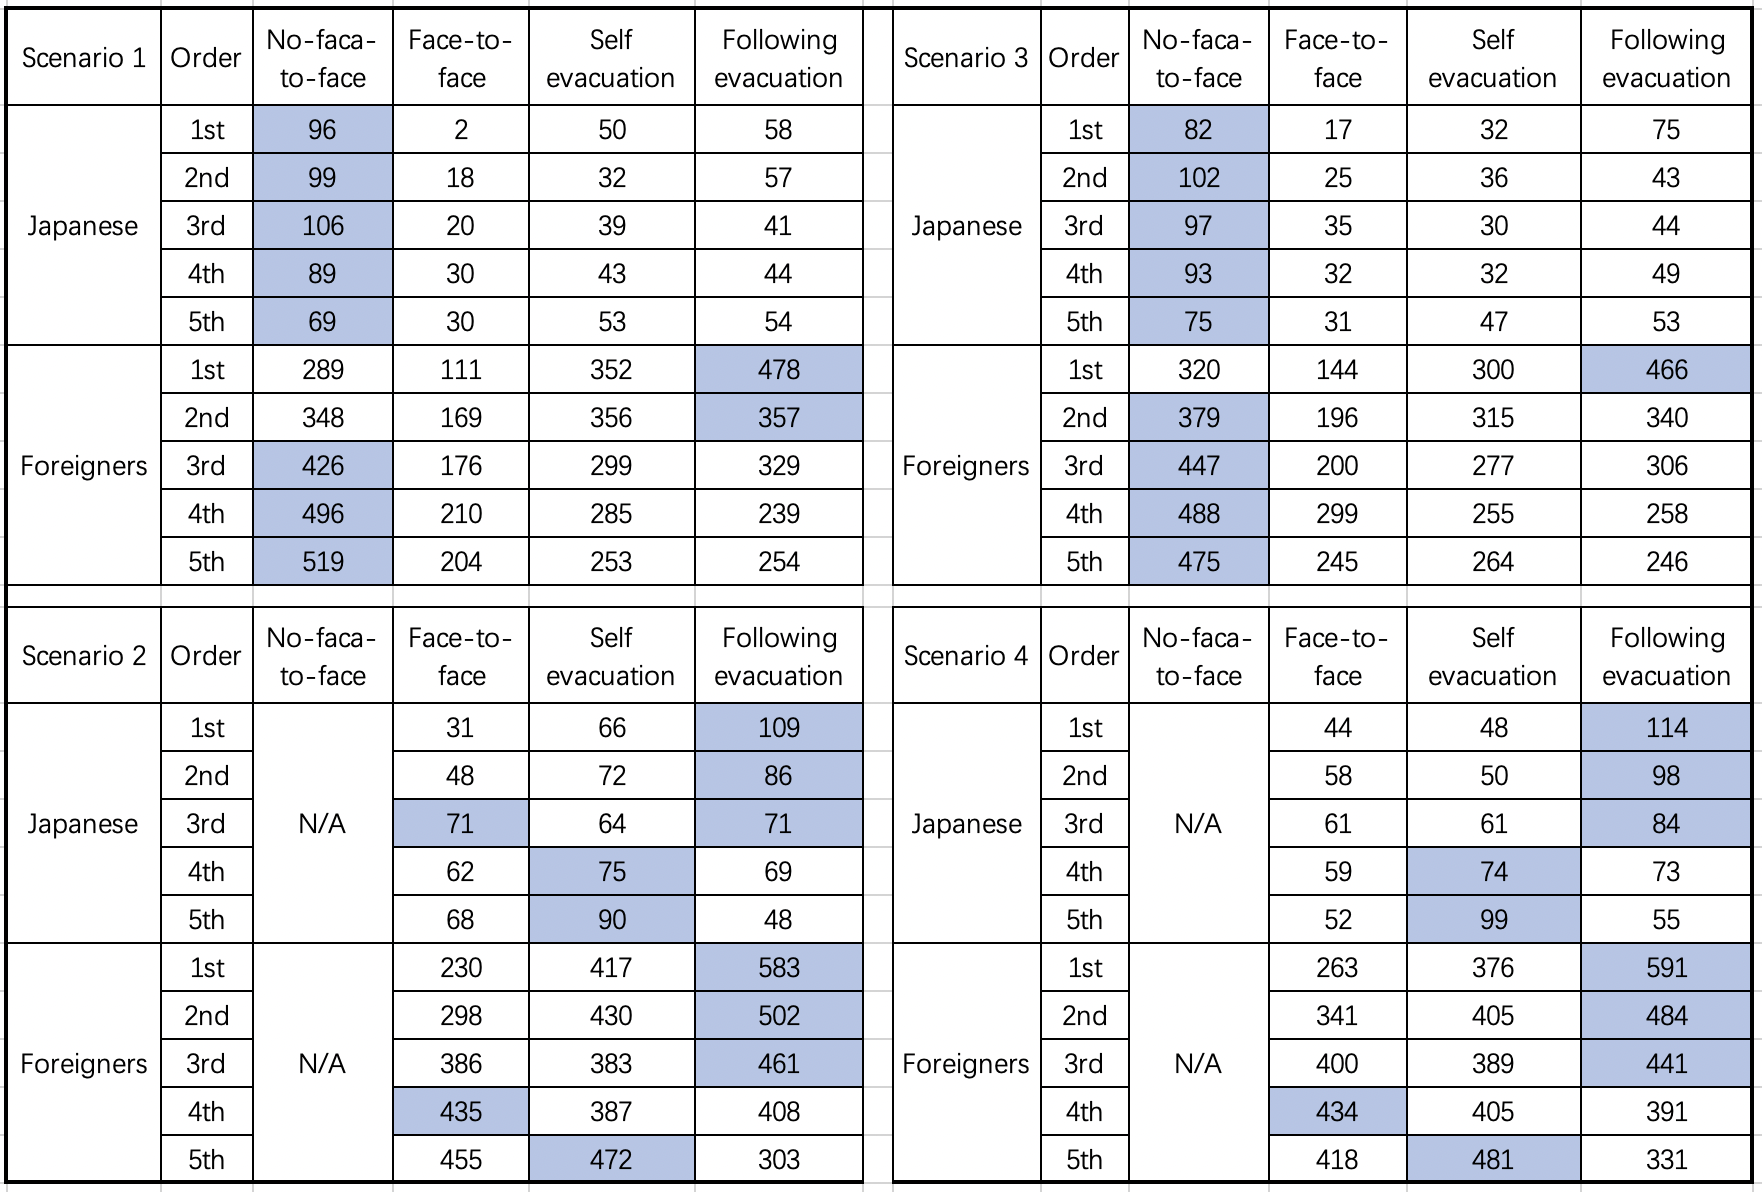
\includegraphics[width=\linewidth]{Figure/Figure28.jpg}
  \centering
  \caption{Summary of Sankey diagram data}
  \label{fig28}
\end{figure*}
%\fi

We can learn from the data that No-face-to-face information seeking is more common than face-to-face information seeking. In the top three actions, following evacuation guidance behaviors are more common than self-evacuation behaviors. 

On the other hand, when the internet and telephone are available, Japanese prefer to take No-face-to-face information-seeking behaviors, while foreign visitors prefer to take following evacuation guidance behavior first, then trend to take No-face-to-face information-seeking behaviors. 

When the internet and phone are unavailable, both Japanese and foreign visitors show similar behavior. Both Japanese and foreigners prefer to take following evacuation guidance behaviors first. However, there are some differences in the behaviors that followed. Self-evacuation behaviors are preferred by the Japanese, while foreigners prefer face-to-face information-seeking behaviors before self-evacuation behaviors.

We can more clearly see the differences between foreign visitors and Japanese when we attribute specific actions to behavior patterns. The most common actions among Japanese in scenarios 1 and 3 are all No-face-to-face information seeking, but the most common behaviors among foreign tourists are following evacuation guidance behaviors, followed by No-face-to-face information seeking. 

I also used the Sankey diagram to analyze the flow of respondents' response actions in each country. The results are shown in \crefrange{fig32}{fig36}. But from the graph we can actually hardly see the difference, basically, the action selection is similar in terms of ratio for each cis. This proves that there is little variability among foreigners and people's actions are not influenced by differences in home country nationality.

\begin{figure*}[h]
  \begin{subfigure}{0.5\textwidth}
    \centering
    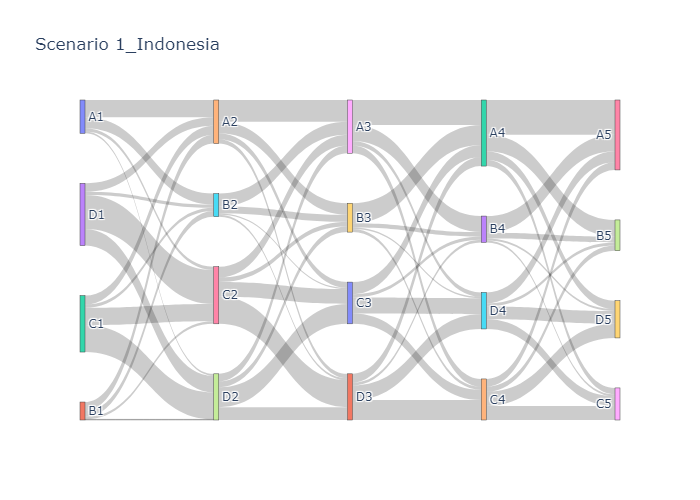
\includegraphics[width=\textwidth]{Figure/figure32a.png}
    \caption{In scenario 1}
    \label{fig32a}
  \end{subfigure}
  \begin{subfigure}{0.5\textwidth}
    \centering
    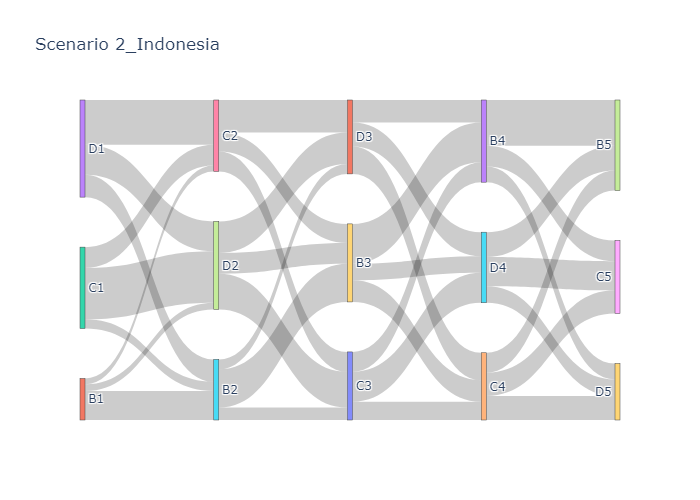
\includegraphics[width=\linewidth]{Figure/figure32b.png}
    \caption{In scenario 2}
    \label{fig32b}
  \end{subfigure}
  \begin{subfigure}{0.5\textwidth}
    \centering
    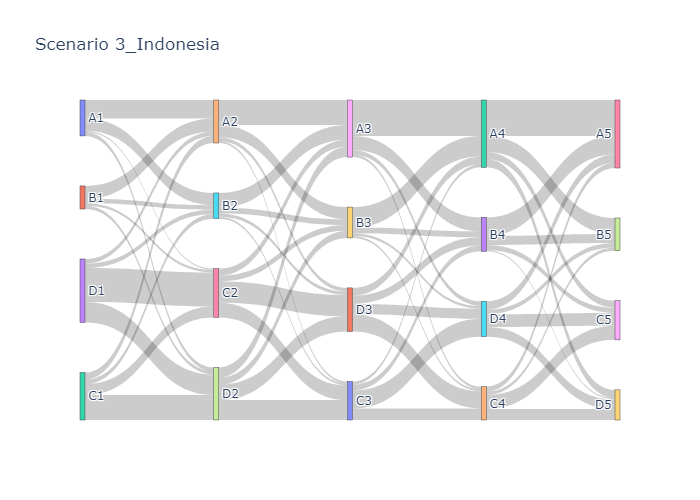
\includegraphics[width=\linewidth]{Figure/figure32c.png}
    \caption{In scenario 3}
    \label{fig32c}
  \end{subfigure}
  \begin{subfigure}{0.5\textwidth}
    \centering
    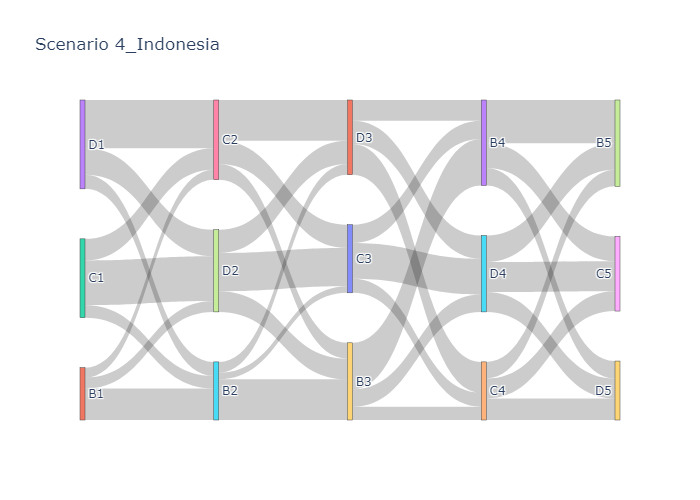
\includegraphics[width=\linewidth]{Figure/figure32d.png}
    \caption{In scenario 4}
    \label{fig32d}
  \end{subfigure}
  \caption{ Sankey diagram of people from Indonesia }
  \label{fig32}
\end{figure*}

\begin{figure*}[h]
  \begin{subfigure}{0.5\textwidth}
    \centering
    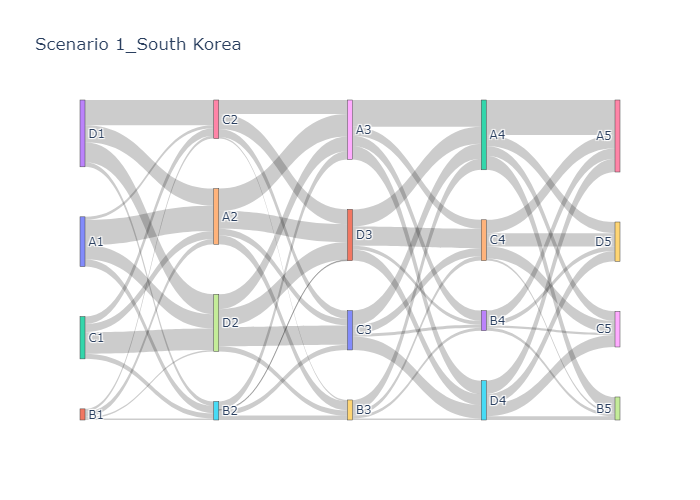
\includegraphics[width=\textwidth]{Figure/figure33a.png}
    \caption{In scenario 1}
    \label{fig33a}
  \end{subfigure}
  \begin{subfigure}{0.5\textwidth}
    \centering
    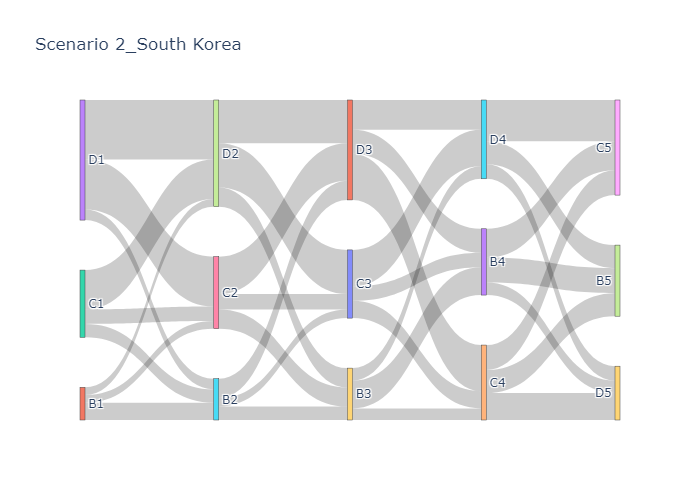
\includegraphics[width=\linewidth]{Figure/figure33b.png}
    \caption{In scenario 2}
    \label{fig33b}
  \end{subfigure}
  \begin{subfigure}{0.5\textwidth}
    \centering
    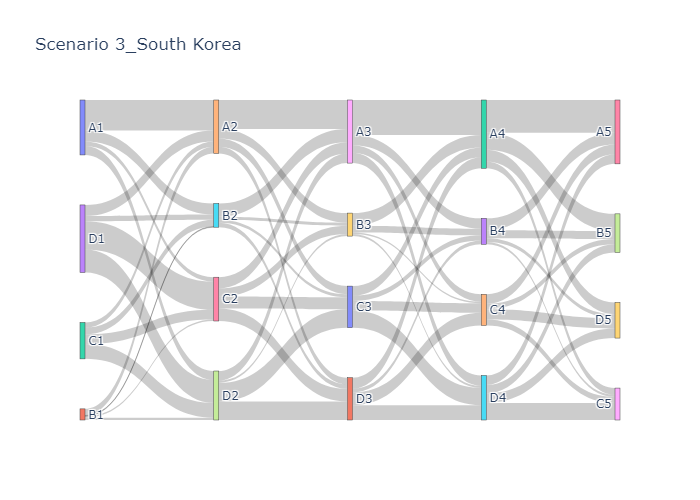
\includegraphics[width=\linewidth]{Figure/figure33c.png}
    \caption{In scenario 3}
    \label{fig33c}
  \end{subfigure}
  \begin{subfigure}{0.5\textwidth}
    \centering
    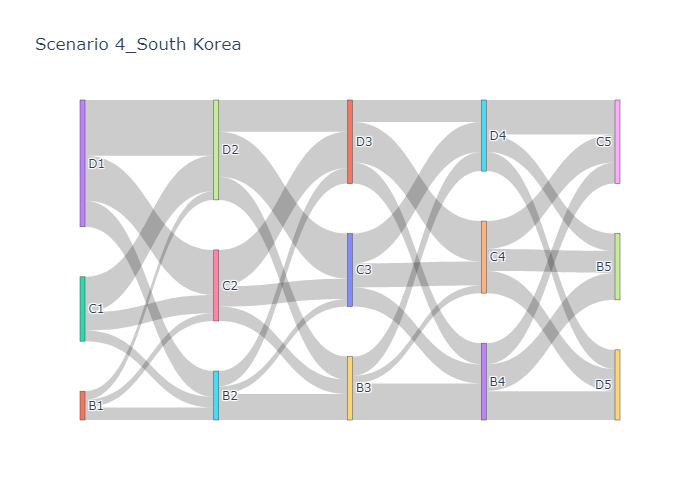
\includegraphics[width=\linewidth]{Figure/figure33d.png}
    \caption{In scenario 4}
    \label{fig33d}
  \end{subfigure}
  \caption{ Sankey diagram of people from South Korea }
  \label{fig33}
\end{figure*}

\begin{figure*}[h]
  \begin{subfigure}{0.5\textwidth}
    \centering
    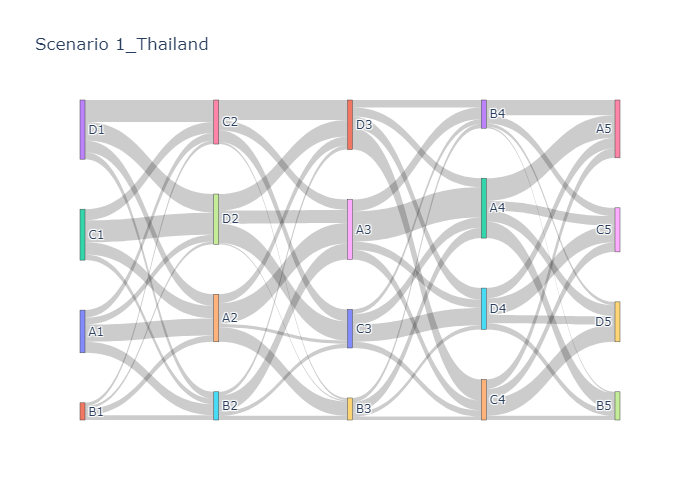
\includegraphics[width=\textwidth]{Figure/figure34a.png}
    \caption{In scenario 1}
    \label{fig34a}
  \end{subfigure}
  \begin{subfigure}{0.5\textwidth}
    \centering
    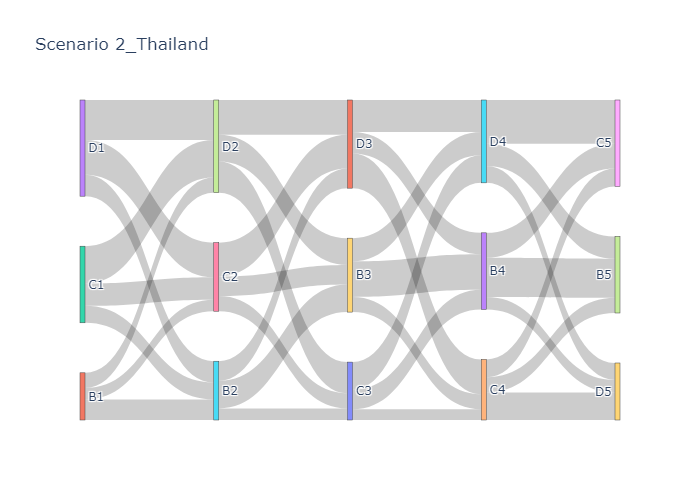
\includegraphics[width=\linewidth]{Figure/figure34b.png}
    \caption{In scenario 2}
    \label{fig34b}
  \end{subfigure}
  \begin{subfigure}{0.5\textwidth}
    \centering
    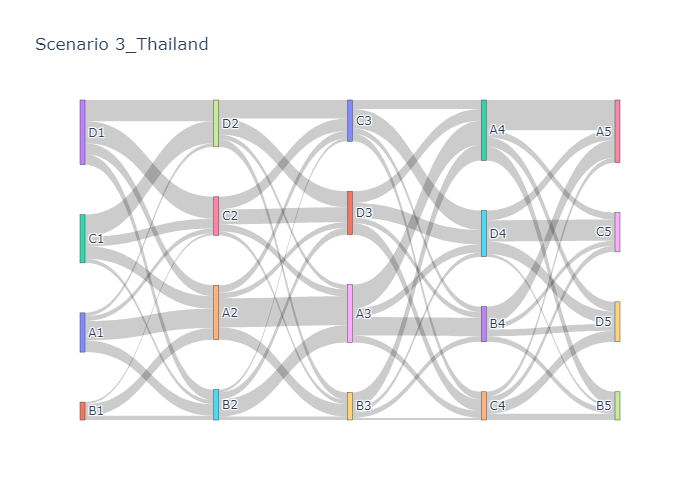
\includegraphics[width=\linewidth]{Figure/figure34c.png}
    \caption{In scenario 3}
    \label{fig34c}
  \end{subfigure}
  \begin{subfigure}{0.5\textwidth}
    \centering
    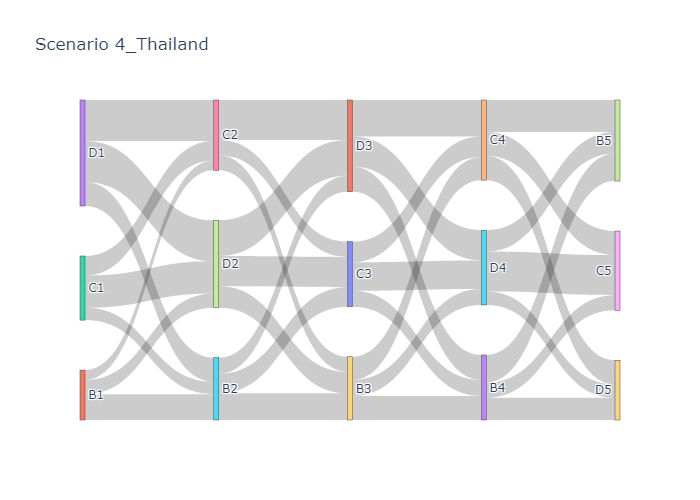
\includegraphics[width=\linewidth]{Figure/figure34d.png}
    \caption{In scenario 4}
    \label{fig34d}
  \end{subfigure}
  \caption{ Sankey diagram of people from Thailand}
  \label{fig34}
\end{figure*}

\begin{figure*}[h]
  \begin{subfigure}{0.5\textwidth}
    \centering
    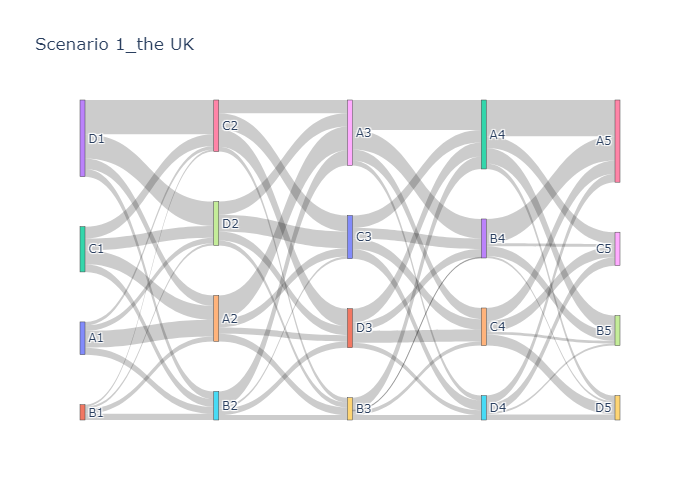
\includegraphics[width=\textwidth]{Figure/figure35a.png}
    \caption{In scenario 1}
    \label{fig35a}
  \end{subfigure}
  \begin{subfigure}{0.5\textwidth}
    \centering
    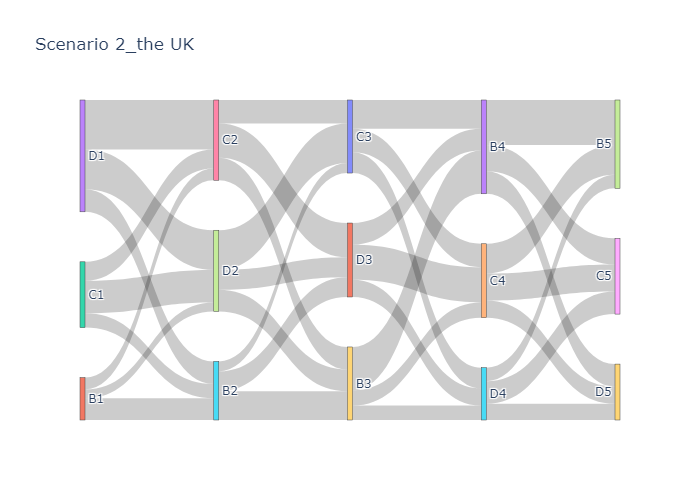
\includegraphics[width=\linewidth]{Figure/figure35b.png}
    \caption{In scenario 2}
    \label{fig35b}
  \end{subfigure}
  \begin{subfigure}{0.5\textwidth}
    \centering
    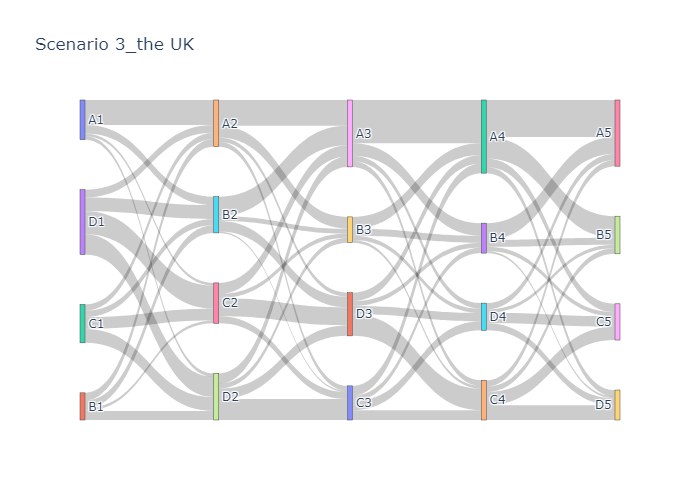
\includegraphics[width=\linewidth]{Figure/figure35c.png}
    \caption{In scenario 3}
    \label{fig35c}
  \end{subfigure}
  \begin{subfigure}{0.5\textwidth}
    \centering
    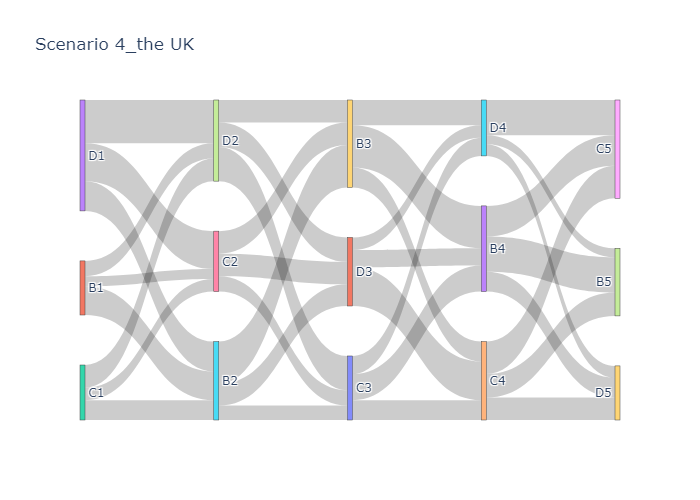
\includegraphics[width=\linewidth]{Figure/figure35d.png}
    \caption{In scenario 4}
    \label{fig35d}
  \end{subfigure}
  \caption{ Sankey diagram of people from the UK}
  \label{fig35}
\end{figure*}


\begin{figure*}[h]
  \begin{subfigure}{0.5\textwidth}
    \centering
    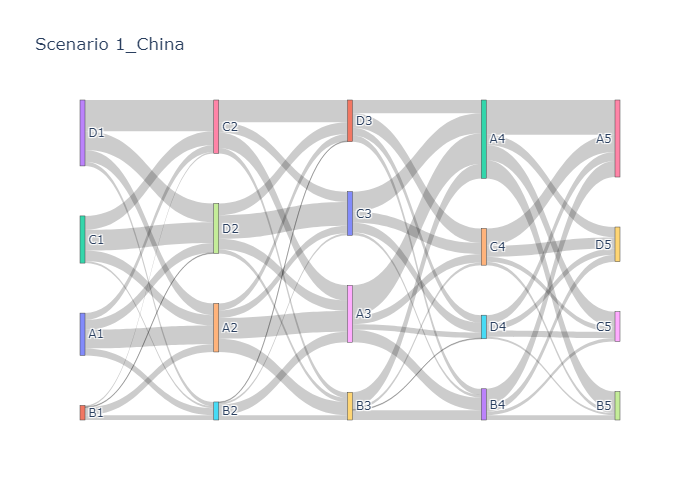
\includegraphics[width=\textwidth]{Figure/figure36a.png}
    \caption{In scenario 1}
    \label{fig36a}
  \end{subfigure}
  \begin{subfigure}{0.5\textwidth}
    \centering
    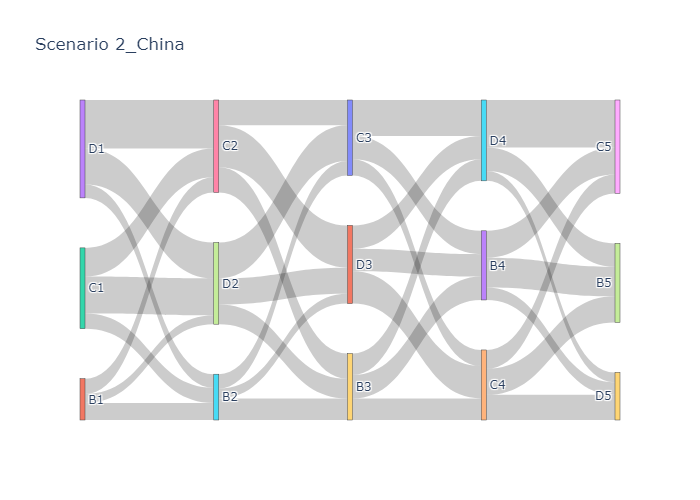
\includegraphics[width=\linewidth]{Figure/figure36b.png}
    \caption{In scenario 2}
    \label{fig36b}
  \end{subfigure}
  \begin{subfigure}{0.5\textwidth}
    \centering
    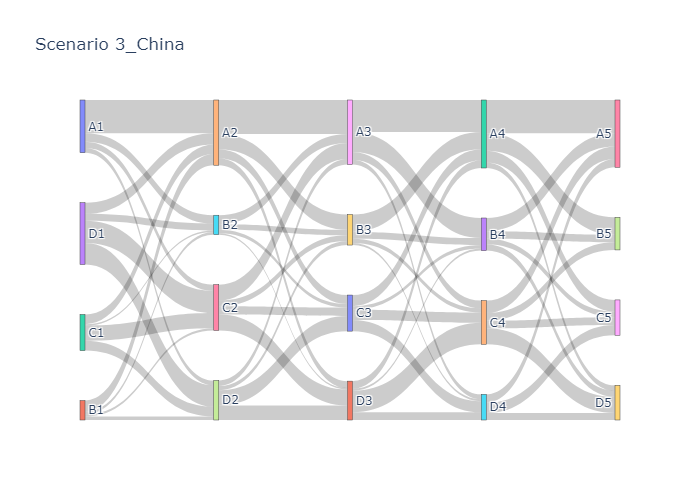
\includegraphics[width=\linewidth]{Figure/figure36c.png}
    \caption{In scenario 3}
    \label{fig36c}
  \end{subfigure}
  \begin{subfigure}{0.5\textwidth}
    \centering
    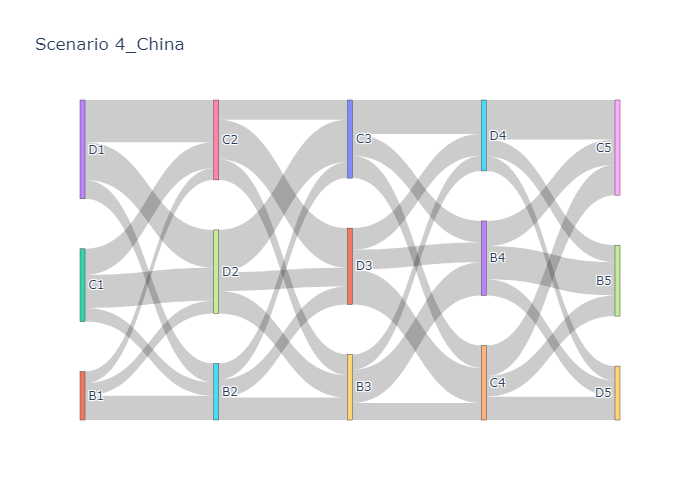
\includegraphics[width=\linewidth]{Figure/figure36d.png}
    \caption{In scenario 4}
    \label{fig36d}
  \end{subfigure}
  \caption{ Sankey diagram of people from China}
  \label{fig36}
\end{figure*}


